\documentclass[12pt]{article}
%\usepackage[utf8]{inputenc}
%\documentclass[UTF8]{ctexart}
%\usepackage[UTF8, heading = false, scheme = plain]{ctex}
\usepackage{geometry}
%geometry{a4paper,scale=0.9}
\geometry{a4paper,left=1cm,right=1cm,top=1cm,bottom=2cm}
\usepackage{amsfonts}
\usepackage{color}
\usepackage{url}
%\usepackage{biblatex}
\usepackage{amsmath}
\usepackage{amssymb}
\usepackage{latexsym}
\usepackage[linesnumbered,ruled,lined]{algorithm2e}
\usepackage{cite}
%\addbibresource{ref.bib}
%\bibliography{ref.bib}
\usepackage{caption}
\usepackage{graphicx, subfig}
\usepackage{float}
%\usepackage[fontset=ubuntu]{ctex}
%\usepackage{fontspec}
\usepackage{xeCJK}
%\usepackage[colorlinks,
%anchorcolor=black,
%citecolor=black]{hyperref}
%\setmainfont{SimSun}
\usepackage[section]{placeins}
\usepackage{enumitem}
\usepackage{framed}
\usepackage[framemethod=TikZ]{mdframed}
\usepackage{indentfirst}
\usepackage{setspace}%使用间距宏包
\linespread{1.5}

\title{推荐系统脉络\cite{Deep_Learning_Recommender_System}}
\author{leolinuxer}
%\date{June 2020}

\begin{document}
%\setlength{\parindent}{0pt}
\maketitle
\tableofcontents

\part{推荐系统的概念}
\section{前深度学习时代CTR预估模型的演化之路}
\begin{figure}[H]
    \centering
    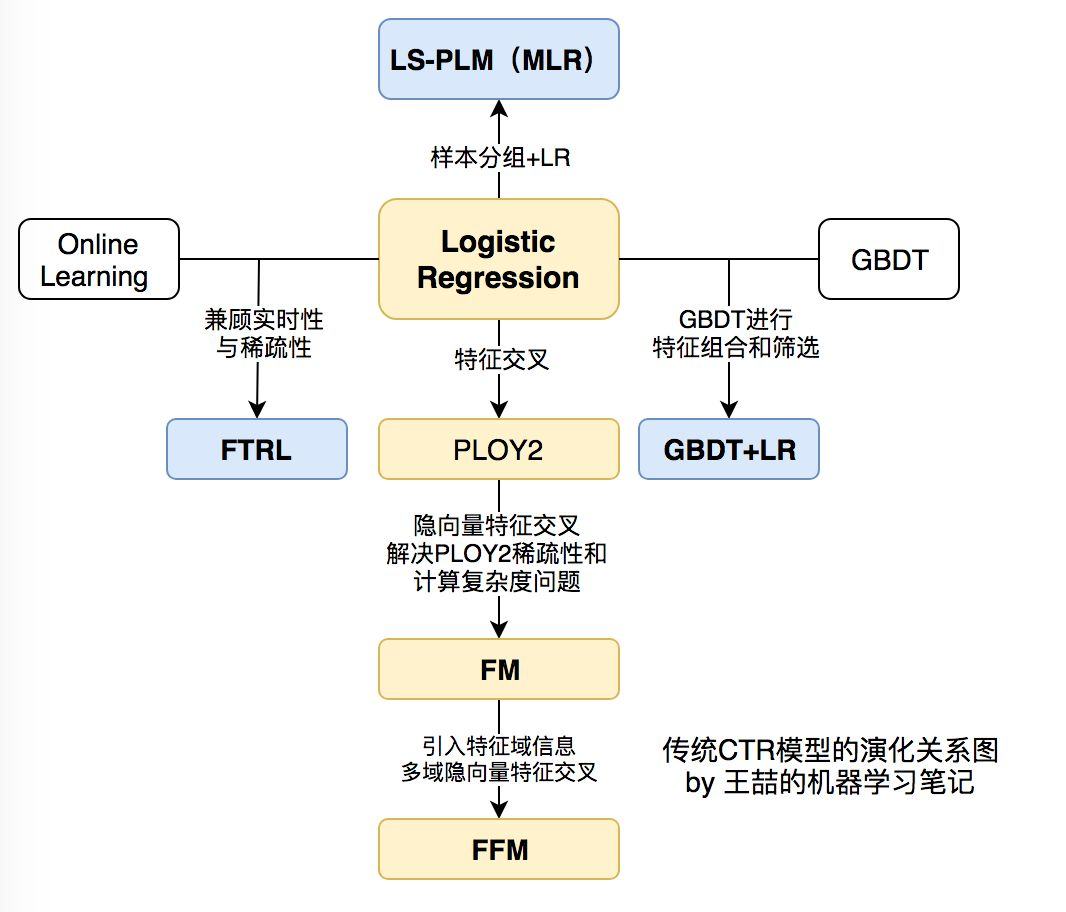
\includegraphics[width=1\textwidth]{fig/Traditional_CTR_Model_Evolution.jpg}
\end{figure}

看到上面的关系图,有经验的同学可能已经对各模型的细节和特点如数家珍了。中间位置的LR模型向四个方向的延伸分别代表了传统CTR模型演化的四个方向。
\begin{itemize}
\setlength{\itemsep}{0pt}
\setlength{\parsep}{0pt}
\setlength{\parskip}{0pt}
    \item 向下为了解决\textbf{特征交叉}的问题,演化出PLOY2,FM,FFM等模型;
    \item 向右为了使用模型化、自动化的手段解决之前\textbf{特征工程}的难题,Facebook将LR与GBDT进行结合,提出了GBDT+LR组合模型;
    \item 向左Google从\textbf{online learning}的角度解决模型时效性的问题,提出了FTRL;
    \item 向上阿里基于\textbf{样本分组}的思路增加模型的非线性,提出了LS-PLM(MLR)模型。
\end{itemize}

\subsection{LR——CTR模型的核心和基础}
位于正中央的是当之无愧的Logistic Regression。仍记得2012年我刚进入计算广告这个行业的时候,各大中小公司的主流CTR模型无一例外全都是LR模型。LR模型的流行是有三方面原因的,一是数学形式和含义上的支撑;二是人类的直觉和可解释性的原因;三是工程化的需要。

\subsubsection{逻辑回归的数学基础}
逻辑回归作为广义线性模型的一种,\textbf{它的假设是因变量 $y$ 服从伯努利分布}。那么在点击率预估这个问题上,“点击”这个事件是否发生就是模型的因变量 $y$。而用户是否点击广告这个问题是一个经典的掷偏心硬币问题,因此CTR模型的因变量显然应该服从伯努利分布。所以采用LR作为CTR 模型是符合“点击”这一事件的物理意义的。

与之相比较,线性回归(Linear Regression)作为广义线性模型的另一个特例,其\textbf{假设是因变量 $y$ 服从高斯分布},这明显不是点击这类二分类问题的数学假设。

在了解LR的数学理论基础后,其数学形式就不再是空中楼阁了,具体的形式如下:
$$
h_\theta(x) = \frac{1}{1 + e^{-\theta^Tx}}
$$

其中 $x$ 是输入向量,$\theta$ 是我们要学习的参数向量。结合CTR模型的问题来说,$x$ 就是输入的特征向量,$h(x)$ 就是我们最终希望得到的点击率。

\subsubsection{人类的直觉和可解释性}
直观来讲,LR模型目标函数的形式就是各特征的加权和,再施以sigmoid函数。忽略其数学基础(虽然这是其模型成立的本质支撑),仅靠人类的直觉认知也可以一定程度上得出使用LR作为CTR模型的合理性。

使用各特征的加权和是为了综合不同特征对CTR的影响,而由于不同特征的重要程度不一样,所以为不同特征指定不同的权重来代表不同特征的重要程度。最后要套上sigmoid函数,正是希望其值能够映射到0-1之间,使其符合CTR的物理意义。

LR如此符合人类的直觉认知显然有其他的好处,就是模型具有极强的可解释性,算法工程师们可以轻易的解释哪些特征比较重要,在CTR模型的预测有偏差的时候,也可以轻易找到哪些因素影响了最后的结果,如果你有跟运营、产品一起工作的经验的话,更会知道可解释性强是一个模型多么优秀的“品质”。

\subsubsection{工程化的需要}
在互联网公司每天动辄TB级别的数据面前,模型的训练开销就异常重要了。在GPU尚未流行开来的2012年之前,LR模型也凭借其易于并行化、模型简单、训练开销小等特点占据着工程领域的主流。囿于工程团队的限制,即使其他复杂模型的效果有所提升,在没有明显beat LR之前,公司也不会贸然加大计算资源的投入升级CTR模型,这是LR持续流行的另一重要原因。

\subsection{POLY2——特征交叉的开始}
但LR的表达能力毕竟是非常初级的。由于LR仅使用单一特征,无法利用高维信息,在“辛普森悖论”现象的存在下,只用单一特征进行判断,甚至会得出错误的结论。

针对这个问题,当时的算法工程师们经常采用手动组合特征,再通过各种分析手段筛选特征的方法。但这个方法无疑是残忍的,完全不符合“懒惰是程序员的美德”这一金科玉律。更遗憾的是,人类的经验往往有局限性,程序员的时间和精力也无法支撑其找到最优的特征组合。因此采用 PLOY2模型进行特征的“暴力”组合成为了可行的选择。
$$
\phi_{\text{Poly2}}(\mathbf{w}, \mathbf{x}) = \sum_{j_1=1}^n\sum_{j_2 = j_1 + 1}^n w_h(j_1, j_2)x_{j_1}x_{j_2}
$$

在上面POLY2二阶部分的目标函数中(上式省略一阶部分和sigmoid函数的部分),我们可以看到POLY2对所有特征进行了两两交叉,并对所有的特征组合赋予了权重 $w_h(j_1, j_2)$。POLY2通过暴力组合特征的方式一定程度上解决了特征组合的问题。并且由于本质上仍是线性模型,其训练方法与LR并无区别,便于工程上的兼容。

但POLY2这一模型同时存在着两个巨大的缺陷:(1) 由于在处理互联网数据时,经常采用one-hot的方法处理id类数据,致使特征向量极度稀疏,POLY2进行无选择的特征交叉使原本就非常稀疏的特征向量更加稀疏,使得大部分交叉特征的权重缺乏有效的数据进行训练,无法收敛;(2) 权重参数的数量由 $n$ 直接上升到 $n^2$,极大增加了训练复杂度。

\subsubsection{FM——隐向量特征交叉}
为了解决POLY2模型的缺陷,2010年德国康斯坦茨大学的Steffen Rendle提出了FM(Factorization Machine)。
$$
\phi_{\text{FM}}(\mathbf{w}, \mathbf{x}) = \sum_{j_1=1}^n\sum_{j_2 = j_1 + 1}^n (\mathbf{w}_{j_1} \cdot \mathbf{w}_{j_2})x_{j_1}x_{j_2}
$$

从 FM 的目标函数的二阶部分中我们可以看到,相比 POLY2,主要区别是用两个向量的内积 $\mathbf{w}_{j_1} \cdot \mathbf{w}_{j_2}$取代了单一的权重 $w_h(j_1, j_2)$。具体来说,FM为每个特征学习了一个隐权重向量(latent vector),在特征交叉时,使用两个特征隐向量的内积作为交叉特征的权重。

通过引入特征隐向量的方式,直接把原先 $n^2$ 级别的权重数量减低到了 $n*k$($k$为隐向量维度,$n >> k$)。在训练过程中,又可以通过转换目标函数形式的方法,使 FM 的训练复杂度进一步降低到 $n*k$ 级别。相比POLY2极大降低训练开销。

\textbf{隐向量的引入还使得FM比POLY2能够更好的解决数据稀疏性的问题}。举例来说,我们有两个特征,分别是channel和brand,一个训练样本的feature组合是(ESPN, Adidas),在POLY2中,只有当ESPN和Adidas同时出现在一个训练样本中时,模型才能学到这个组合特征对应的权重。而在FM中,ESPN的隐向量也可以通过(ESPN, Gucci)这个样本学到,Adidas的隐向量也可以通过(NBC, Adidas)学到,这大大降低了模型对于数据稀疏性的要求。甚至对于一个从未出现过的特征组合(NBC, Gucci),由于模型之前已经分别学习过NBC和Gucci的隐向量,FM也具备了计算该特征组合权重的能力,这是POLY2无法实现的。也许FM相比POLY2丢失了某些信息的记忆能力,但是泛化能力大大提高,这对于互联网的数据特点是非常重要的。

工程方面,FM同样可以用梯度下降进行学习的特点使其不失实时性和灵活性。相比之后深度学习模型复杂的网络结构,FM比较容易实现的inference过程也使其没有serving的难题。因此FM在2012-2014年前后逐渐成为业界CTR模型的重要选择。

\subsubsection{FFM——引入特征域概念}
2015年,基于FM提出的FFM(Field-aware Factorization Machine ,简称FFM)在多项CTR预估大赛中一举夺魁,并随后被Criteo、美团等公司深度应用在CTR预估,推荐系统领域。相比FM模型,FFM模型主要引入了Field-aware这一概念,使模型的表达能力更强。
$$
\phi_{\text{FFM}}(\mathbf{w}, \mathbf{x}) = \sum_{j_1=1}^n\sum_{j_2 = j_1 + 1}^n (\mathbf{w}_{j_1, f_2} \cdot \mathbf{w}_{j_2, f_1})x_{j_1}x_{j_2}
$$

上式是 FFM 的目标函数的二阶部分。其与 FM 目标函数的区别就在于隐向量由原来的 $w_{j_1}$ 变成了 $w_{j_1, f_2}$  ,这就意味着每个特征对应的不是一个隐向量,而是对应着不同域的一组隐向量,当 $w_{j_1}$ 特征与 $w_{j_2}$ 特征进行交叉时,$x_{j_1}$ 特征会从一组隐向量中挑出与特征 $2_{j_2}$ 的域 $f_2$ 对应的隐向量 $w_{j_1, f_2}$ 进行交叉。同理特征 $x_{j_2}$ 也会用与 $x_{j_1}$ 的域 $f_1$ 对应的隐向量进行交叉。

这里再次强调一下,上面所说的“域”就代表着特征域,域内的特征一般会采用one-hot编码形成one-hot特征向量。

FFM模型学习每个特征在 $f$ 个域上的 $k$ 维隐向量,交叉特征的权重由特征在对方特征域上的隐向量内积得到,权重数量共 $n*k*f$ 个。在训练方面,由于FFM的二次项并不能够像 FM 那样简化,因此其复杂度为 $kn^2$。

相比 FM,FFM 由于引入了 field 这一概念,为模型引入了更多有价值信息,使模型表达能力更强,但与此同时,FFM的计算复杂度上升到$kn^2$,远远大于FM的 $k*n$。

\begin{framed}
理解:比较 Poly2、 FM、FFM

Poly2:对所有特征进行两两交叉,为每种特征组合都学习一个权重;

FM:为每个特征学习一个隐权重向量。在特征交叉时,使用两个特征隐向量的内积作为交叉特征的权重。

FFM:为每个特征学习一个隐权重“矩阵”,矩阵的每一列对应一个域,该列向量为对应的隐权重向量。在特征交叉时,使用两个特征对应域的隐向量的内积作为交叉特征的权重。
\end{framed}

\subsection{CTR模型特征交叉方向的演化}
以上模型实际上是CTR模型朝着特征交叉的方向演化的过程,我们再用图示方法回顾一下从POLY2到FM,再到FFM进行特征交叉方法的不同。

POLY2 模型直接学习每个交叉特征的权重,权重数量共 $n^2$ 个。
\begin{figure}[H]
    \centering
    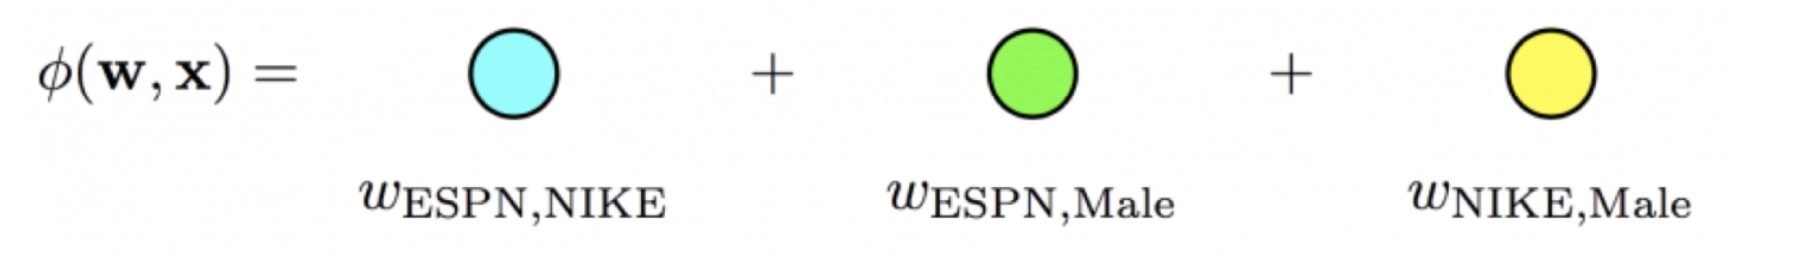
\includegraphics[width=1\textwidth]{fig/CTR_Comparison_Poly2.png}
\end{figure}

FM 模型学习每个特征的 $k$ 维隐向量,交叉特征由相应特征隐向量的内积得到,权重数量共 $n*k$ 个。
\begin{figure}[H]
    \centering
    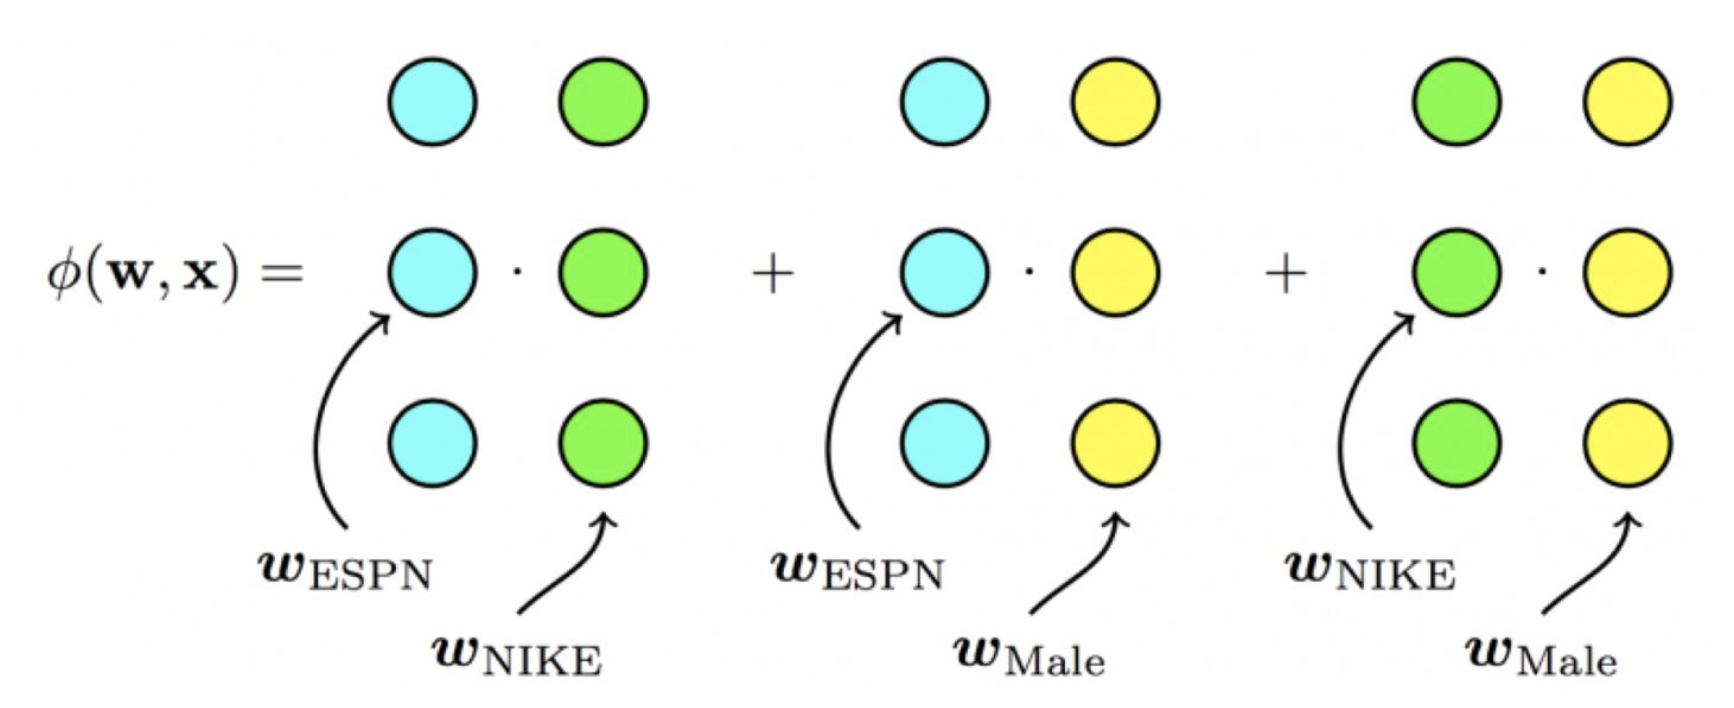
\includegraphics[width=1\textwidth]{fig/CTR_Comparison_FM.png}
\end{figure}

FFM 模型引入了特征域这一概念,在做特征交叉时,每个特征选择与对方域对应的隐向量做内积运算得到交叉特征的权重。参数数量共 $n*k*f$个。
\begin{figure}[H]
    \centering
    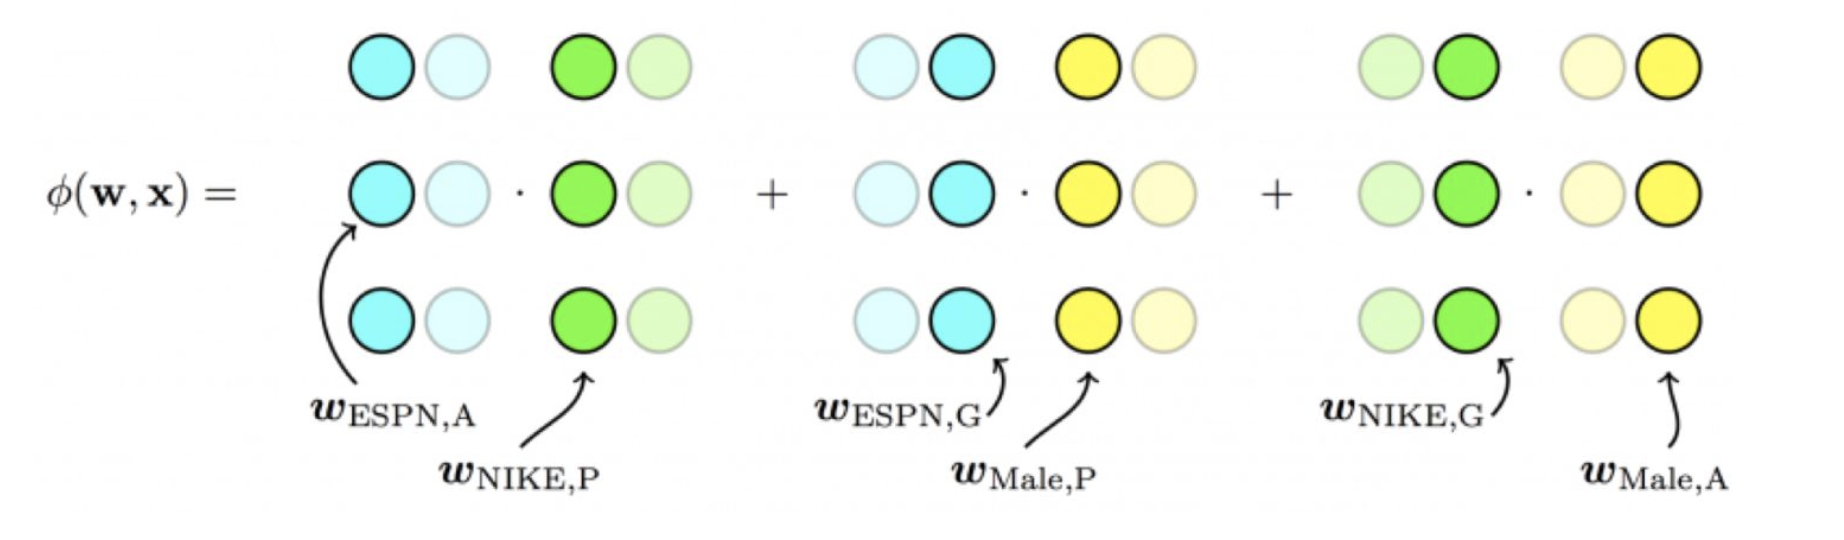
\includegraphics[width=1\textwidth]{fig/CTR_Comparison_FFM.png}
\end{figure}

\subsection{GBDT+LR——特征工程模型化的开端}
FFM模型采用引入特征域的方式增强了模型的表达能力,但无论如何,FFM只能够做二阶的特征交叉,如果要继续提高特征交叉的维度,不可避免的会发生组合爆炸和计算复杂度过高的情况。那么有没有其他的方法可以有效的处理高维特征组合和筛选的问题?2014年,Facebook提出了基于GBDT+LR组合模型的解决方案。

简而言之,Facebook提出了一种利用GBDT自动进行特征筛选和组合,进而生成新的离散特征向量,再把该特征向量当作LR模型输入,预估CTR的模型结构。
\begin{figure}[H]
    \centering
    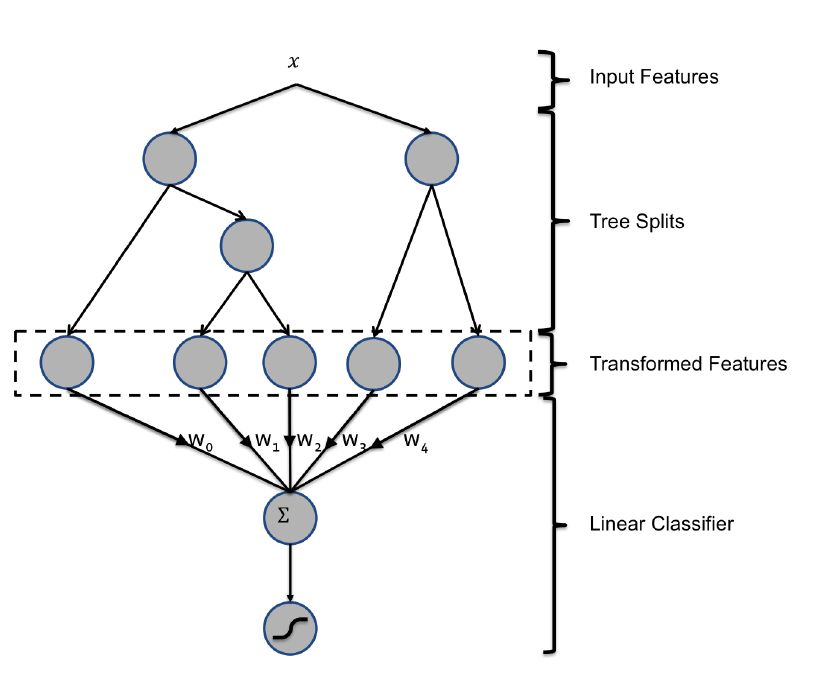
\includegraphics[width=.6\textwidth]{fig/Facebook_GBDT_LR_Feature.jpg}
\end{figure}

大家知道,GBDT 是由多棵回归树组成的树林,后一棵树利用前面树林的结果与真实结果的残差做为拟合目标。每棵树生成的过程是一棵标准的回归树生成过程,因此每个节点的分裂是一个自然的特征选择的过程,而多层节点的结构自然进行了有效的特征组合,也就非常高效的解决了过去非常棘手的特征选择和特征组合的问题。

利用训练集训练好 GBDT 模型之后,就可以利用该模型完成从原始特征向量到新的离散型特征向量的转化。具体过程是这样的,一个训练样本在输入 GBDT 的某一子树后,会根据每个节点的规则最终落入某一叶子节点,那么我们把该叶子节点置为1,其他叶子节点置为0,所有叶子节点组成的向量即形成了该棵树的特征向量,把GBDT所有子树的特征向量连接起来,即形成了后续LR输入的特征向量。

由于决策树的结构特点,事实上,\textbf{决策树的深度就决定了特征交叉的维度}。如果决策树的深度为4,通过三次节点分裂,最终的叶节点实际上是进行了3阶特征组合后的结果,如此强的特征组合能力显然是FM系的模型不具备的。但由于GBDT容易产生过拟合,以及GBDT这种特征转换方式实际上丢失了大量特征的数值信息,因此我们不能简单说GBDT由于特征交叉的能力更强,效果就比FFM好,在模型的选择和调试上,永远都是多种因素综合作用的结果。

GBDT+LR比FM重要的意义在于,\textbf{它大大推进了特征工程模型化这一重要趋势},某种意义上来说,之后深度学习的各类网络结构,以及embedding技术的应用,都是这一趋势的延续。

\subsection{FTRL——天下武功,唯快不破}
FTRL的全称是Follow-the-regularized-Leader,是一种在线实时训练模型的方法,Google在2010年提出了FTRL的思路,2013年实现了FTRL的工程化,之后快速成为online learning的主流方法。与模型演化图中的其他模型不同,FTRL本质上是模型的训练方法。虽然Google的工程化方案是针对LR模型的,但理论上FTRL可以应用在FM,NN等任何通过梯度下降训练的模型上。

为了更清楚的认识FTRL,这里对梯度下降方法做一个简要的介绍,从训练样本的规模角度来说,梯度下降可以分为:batch,mini-batch,SGD(随机梯度下降)三种,batch方法每次都使用全量训练样本计算本次迭代的梯度方向,mini-batch使用一小部分样本进行迭代,而SGD每次只利用一个样本计算梯度。对于online learning来说,为了进行实时得将最新产生的样本反馈到模型中,SGD无疑是最合适的训练方式。

但\textbf{SGD对于互利网广告和推荐的场景来说,有比较大的缺陷,就是难以产生稀疏解}。为什么稀疏解对于CTR模型如此重要呢?

之前我们已经多次强调,由于one hot等id类特征处理方法导致广告和推荐场景下的样本特征向量极度稀疏,维度极高,动辄达到百万、千万量级。为了不割裂特征选择和模型训练两个步骤,如果能够在保证精度的前提下尽可能多的让模型的参数权重为0,那么我们就可以自动过滤掉这些权重为0的特征,生成一个“轻量级”的模型。“轻量级”的模型不仅会使样本部署的成本大大降低,而且可以极大降低模型inference的计算延迟。这就是模型稀疏性的重要之处。

而SGD由于每次迭代只选取一个样本,梯度下降的方向虽然总体朝向全局最优解,但微观上的运动的过程呈现布朗运动的形式,这就导致SGD会使几乎所有特征的权重非零。即使加入L1正则化项,由于CPU浮点运算的结果很难精确的得到0的结果,也不会完全解决SGD稀疏性差的问题。就是在这样的前提下,\textbf{FTRL几乎完美地解决了模型精度和模型稀疏性兼顾的训练问题}。
\begin{figure}[H]
    \centering
    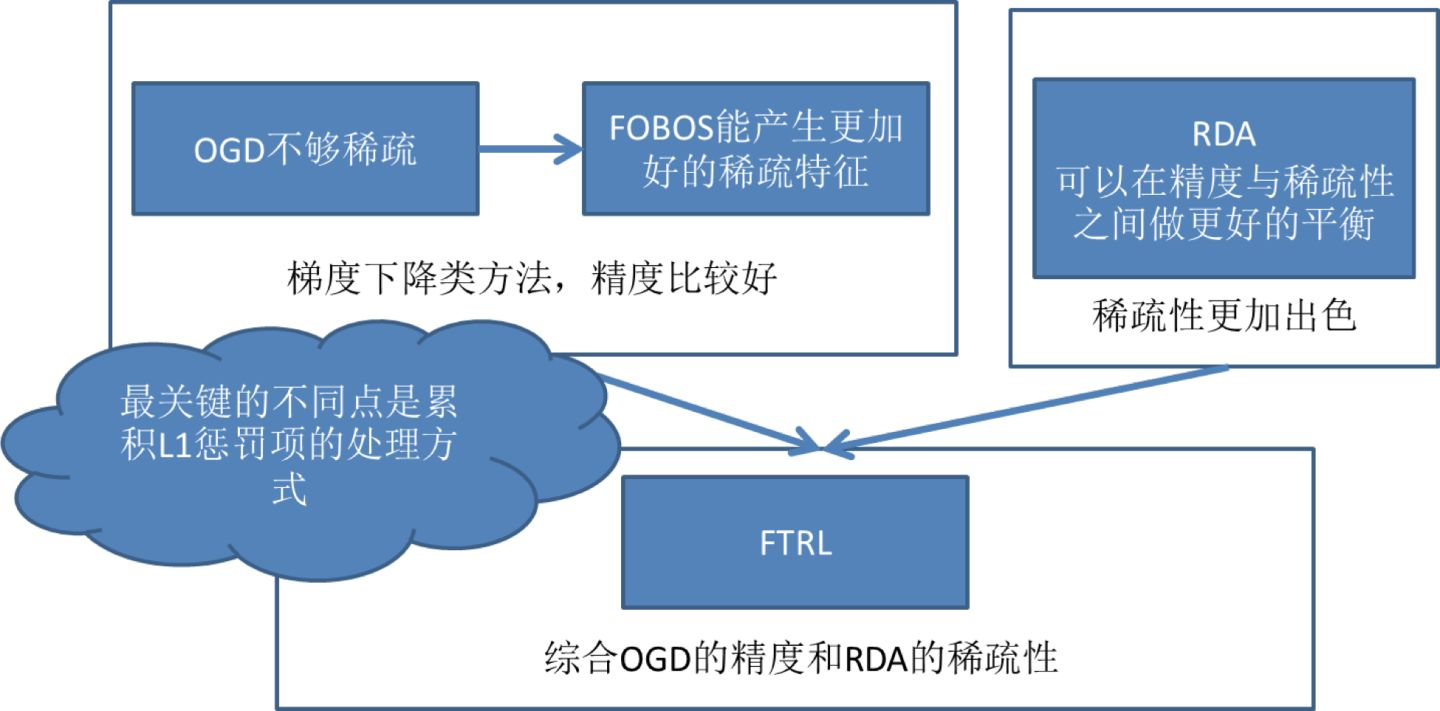
\includegraphics[width=1\textwidth]{fig/FTRL_Evolution.jpg}
\end{figure}

但FTRL的提出也并不是一蹴而就的。如上图所示,FTRL的提出经历了下面几个关键的过程:
\begin{itemize}
\setlength{\itemsep}{0pt}
\setlength{\parsep}{0pt}
\setlength{\parskip}{0pt}
    \item \textbf{从最近简单的SGD到OGD(online gradient descent)},OGD通过引入L1正则化简单解决稀疏性问题;
    \item \textbf{从OGD到截断梯度法},通过暴力截断小数值梯度的方法保证模型的稀疏性,但损失了梯度下降的效率和精度;
    \item \textbf{FOBOS(Forward-Backward Splitting)},google和伯克利对OGD做进一步改进,09年提出了保证精度并兼顾稀疏性的FOBOS方法;
    \item \textbf{RDA}:微软抛弃了梯度下降这条路,独辟蹊径提出了正则对偶平均来进行online learning的方法,其特点是稀疏性极佳,但损失了部分精度。
    \item Google\textbf{综合FOBOS在精度上的优势和RDA在稀疏性上的优势},将二者的形式进行了进一步统一,提出并应用FTRL,使FOBOS和RDA均成为了FTRL在特定条件下的特殊形式。
\end{itemize}

\subsection{LS-PLM——阿里曾经的主流CTR模型}
下面我们从样本pattern本身来入手,介绍阿里的的LS-PLM(Large Scale Piece-wise Linear Model),它的另一个更广为人知的名字是MLR(Mixed Logistic Regression)。MLR模型虽然在2017年才公之于众,但其早在2012年就是阿里主流的CTR模型,并且在深度学习模型提出之前长时间应用于阿里的各类广告场景。

本质上,MLR可以看做是对LR的自然推广,它在LR的基础上采用分而治之的思路,先对样本进行分片,再在样本分片中应用LR进行CTR预估。在LR的基础上加入聚类的思想,其动机其实来源于对计算广告领域样本特点的观察 。

举例来说,如果CTR模型要预估的是女性受众点击女装广告的CTR,显然我们并不希望把男性用户点击数码类产品的样本数据也考虑进来,因为这样的样本不仅对于女性购买女装这样的广告场景毫无相关性,甚至会在模型训练过程中扰乱相关特征的权重。为了让CTR模型对不同用户群体,不用用户场景更有针对性,其实理想的方法是先对全量样本进行聚类,再对每个分类施以LR模型进行CTR预估。MLR的实现思路就是由该动机产生的。
$$
f(x) = \sum_{i=1}^m\pi_i(x) \cdot \eta_i(x) = \sum_{i=1}^m \frac{e^{\mu_i \cdot x}}{\sum_{j=1}^m e^{\mu_j\cdot x}} \cdot \frac{1}{1+e^{-w_i\cdot x}}
$$

MLR目标函数的数学形式如上式,首先用聚类函数 $\pi$ 对样本进行分类(这里的 $\pi$ 采用了softmax函数,对样本进行多分类),再用 LR模型计算样本在分片中具体的 CTR,然后将二者进行相乘后加和。

其中超参数分片数 $m$ 可以较好地平衡模型的拟合与推广能力。当 $m=1$ 时MLR就退化为普通的LR,$m$ 越大模型的拟合能力越强,但是模型参数规模随 $m$ 线性增长,相应所需的训练样本也随之增长。在实践中,阿里给出了 $m$ 的经验值为12。

MLR算法适合于工业级的广告、推荐等大规模稀疏数据场景问题。主要是由于表达能力强、稀疏性高等两个优势

(1). \textbf{端到端的非线性学习}:从模型端自动挖掘数据中蕴藏的非线性模式,省去了大量的人工特征设计,这使得MLR算法可以端到端地完成训练,在不同场景中的迁移和应用非常轻松。

(2). \textbf{稀疏性}:MLR 在建模时引入了L1和L2,1范数,可以使得最终训练出来的模型具有较高的稀疏度,模型的学习和在线预测性能更好。

如果我们用深度学习的眼光来看待MLR这个模型,其在结构上已经很接近由输入层、单隐层、输出层组成的神经网络。所以某种意义上说,MLR也在用自己的方式逐渐逼近深度学习的大门了。

\subsection{深度学习CTR模型的前夜}
2010年FM被提出,特征交叉的概念被引入CTR模型;2012年MLR在阿里大规模应用,其结构十分接近三层神经网络;2014年Facebook用GBDT处理特征,揭开了特征工程模型化的篇章。这些概念都将在深度学习CTR模型中继续应用,持续发光。

另一边,Alex Krizhevsky 2012年提出了引爆整个深度学习浪潮的AlexNet,深度学习的大幕正式拉开,其应用逐渐从图像扩展到语音,再到NLP领域,推荐和广告也必然会紧随其后,投入深度学习的大潮之中。

2016年,随着FNN,Deep\&Wide,Deep crossing等一大批优秀的CTR模型框架的提出,深度学习CTR模型逐渐席卷了推荐和广告领域,成为新一代CTR模型当之无愧的主流。

\section{深度学习推荐模型的演化趋势}
\begin{figure}[H]
    \centering
    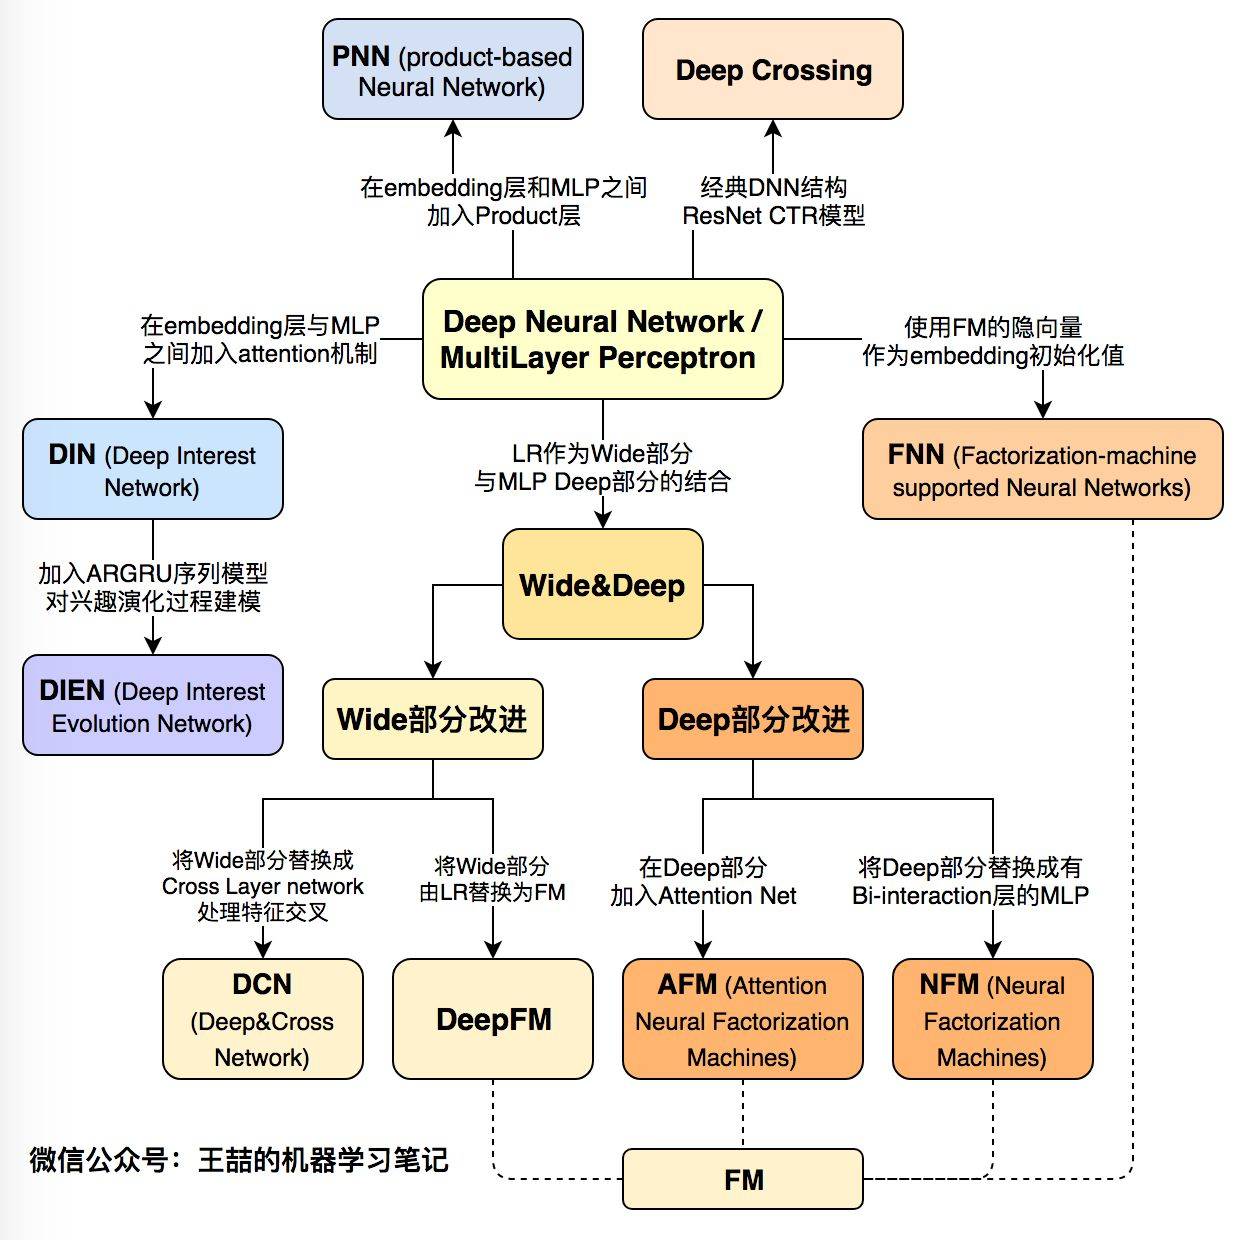
\includegraphics[width=1\textwidth]{fig/Deep_Learning_Reference_System_Evolution.jpg}
\end{figure}

上图中涉及到的主要知识点如下:
\begin{itemize}
\setlength{\itemsep}{0pt}
\setlength{\parsep}{0pt}
\setlength{\parskip}{0pt}
    \item Product 层
    \item AutoEncoder
    \item Attention 机制
    \item ARGRU
    \item Cross Layer Network
    \item Bi-interaction
    \item ……
\end{itemize}

\section{推荐系统的系统架构}
\begin{figure}[H]
    \centering
    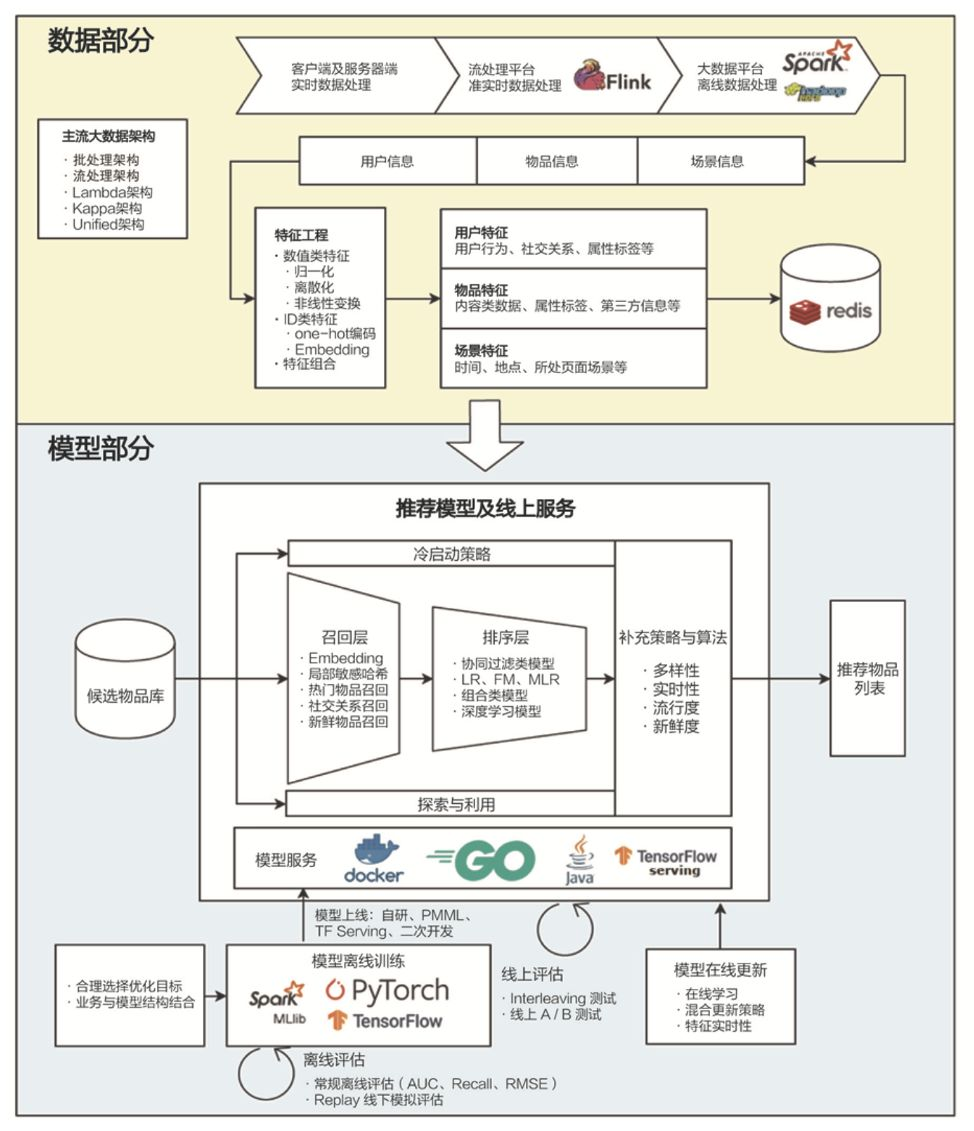
\includegraphics[width=1\textwidth]{fig/Deep_Learning_Refenrence_System_Architecture.jpg}
\end{figure}


\part{推荐系统的工业化应用}
\section{Facebook的经典CTR预估模型}
论文:Practical Lessons from Predicting Clicks on Ads at Facebook

\subsection{用户场景}
论文中的用户场景是一个标准的点击率预估的场景,需要强调的只有一点,因为我们需要利用CTR计算精准的出价、ROI等重要的后续预估值,因此CTR模型的预估值需要是一个\textbf{具有物理意义的精准的CTR,而不是仅仅输出广告排序的高低关系}。所以文中不仅把CTR calibration作为重要的评价指标,更是在最后介绍了模型校正的相关方法。

\subsection{模型结构}
文章提出了一种利用GBDT自动进行特征筛选和组合,进而生成新的feature vector,再把该feature vector当作logistic regression的模型输入,预测CTR的模型结构。
\begin{figure}[H]
    \centering
    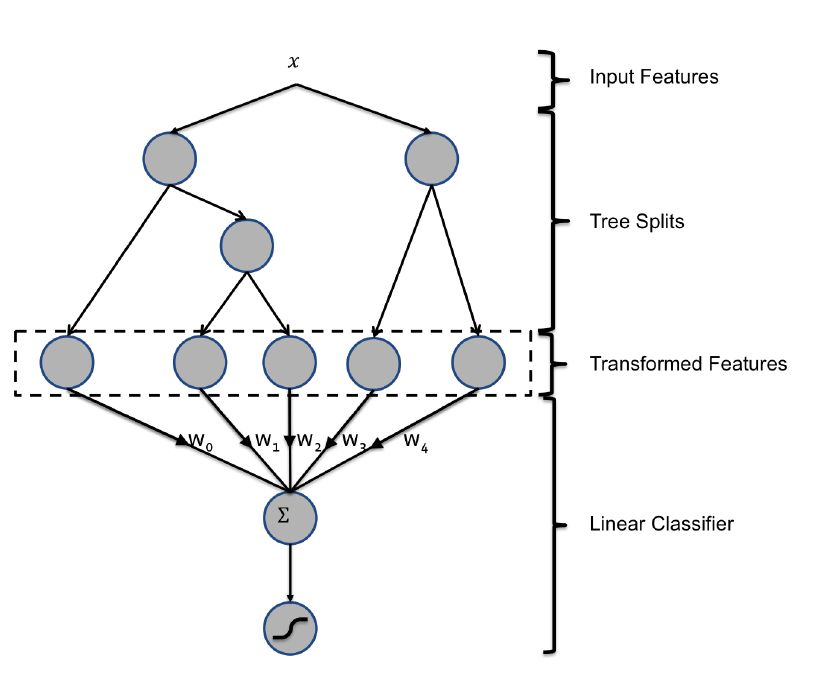
\includegraphics[width=.6\textwidth]{fig/Facebook_GBDT_LR_Feature.jpg}
\end{figure}

这里需要强调的是,\textbf{用GBDT构建特征工程,和利用LR预测CTR两步是独立训练的}。所以自然不存在如何将LR的梯度回传到GBDT这类复杂的问题,而利用LR预测CTR的过程是显然的,在此不再赘述,我们着重讲一讲如何利用GBDT构建新的特征向量。

大家知道,GBDT是由多棵回归树组成的树林,后一棵树利用前面树林的结果与真实结果的残差做为拟合目标。每棵树生成的过程是一棵标准的回归树生成过程,因此每个节点的分裂是一个自然的特征选择的过程,而多层节点的结构自然进行了有效的特征组合,也就非常高效的解决了过去非常棘手的特征选择和特征组合的问题。

我们利用训练集训练好GBDT模型,之后就可以利用该模型构建特征工程。具体过程是这样的,一个样本在输入GBDT的某一子树后,会根据每个节点的规则最终落入某一叶子节点,那么我们把该叶子节点置为1,其他叶子节点置为0,所有叶子节点组成的向量即形成了该棵树的特征向量,把GBDT所有子树的特征向量concatenate起来,即形成了后续LR输入的特征向量。

举例来说,比如GBDT由三颗子树构成,每个子树有4个叶子节点,一个训练样本进来后,先后落到了“子树1”的第3个叶节点中,那么特征向量就是[0,0,1,0],“子树2”的第1个叶节点,特征向量为[1,0,0,0],“子树3”的第4个叶节点,特征向量为[0,0,0,1],最后concatenate所有特征向量,形成的最终的特征向量为[0,0,1,0,1,0,0,0,0,0,0,1],我们再把该向量作为LR的输入,预测CTR。

引入了GBDT+LR的模型后,相比单纯的LR和GBDT,提升效果是非常显著的。从论文中可以看到,混合模型比单纯的LR或Trees模型在loss上减少了3%。

该模型的优势我们上面已经提到,即可以自动进行特征组合和特征筛选,但在实践过程中,模型的缺陷也比较明显,相比FTRL,FM,NN等能够通过梯度下降训练的模型来说,\textbf{GBDT缺乏online learning的能力,因此我们往往只能相隔一天甚至几天才能够update GBDT模型,势必影响模型的实效性},那么Facebook是如何解决模型更新的问题的呢?

\subsection{模型的实效性问题和更新策略}
虽然我们的直觉是模型的训练时间和serving时间之间的间隔越短,模型的效果越好,但为了证明这一点,facebook的工程师还是做了一组实效性的实验,在结束模型的训练之后,观察了其后6天的模型loss(这里采用normalized entropy作为loss)
\begin{figure}[H]
    \centering
    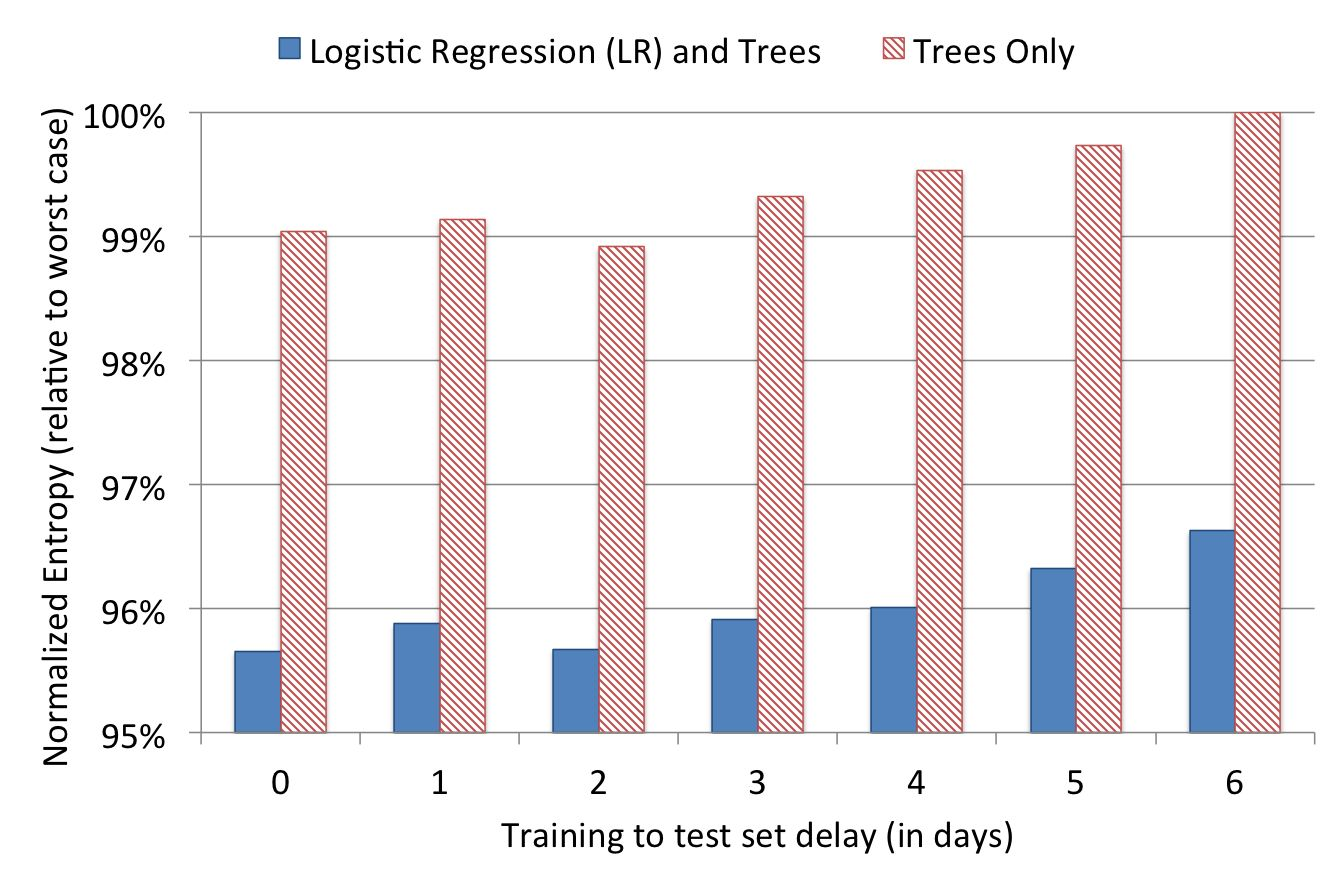
\includegraphics[width=.6\textwidth]{fig/Facebook_GTDT_LR_Training_Delay.jpg}
    \caption{模型更新延迟与loss的关系}
\end{figure}

可以看出,模型的loss在第0天之后有所上升,特别是第2天过后显著上升。因此daily update的模型相比weekly update的模型效果肯定是有大幅提升的。

但囿于facebook巨大的数据量以及GBDT较难实施并行化的原因,GBDT的更新时间往往超过24小时,所以为了兼顾data freshness和客观的工程要求,facebook采取了下面的模型更新方法:

The boosted decision trees can be trained daily or every couple of days, but the linear classifier can be trained in near real-time by using some flavor of online learning.

就是说GBDT的部分几天更新一次,而LR的部分进行准实时的更新,这无疑是很好的工程实践经验。时至今日,我们已经开始使用大量不同的embedding方法进行特征编码,facebook当时的做法也对我们现在的工程实践有重要的参考价值。因为大量深度学习embedding方法的更新计算开销也非常大,但对实效性要求并不高,我们也完全可以低频更新embedding,高频或实时更新基于embedding特征的LR,NN等预测模型。

\subsection{facebook的实时数据流架构}

为了实现模型的准实时训练,facebook专门介绍了其基于Scribe的数据流架构,文中称其为online data joiner。
\begin{figure}[H]
    \centering
    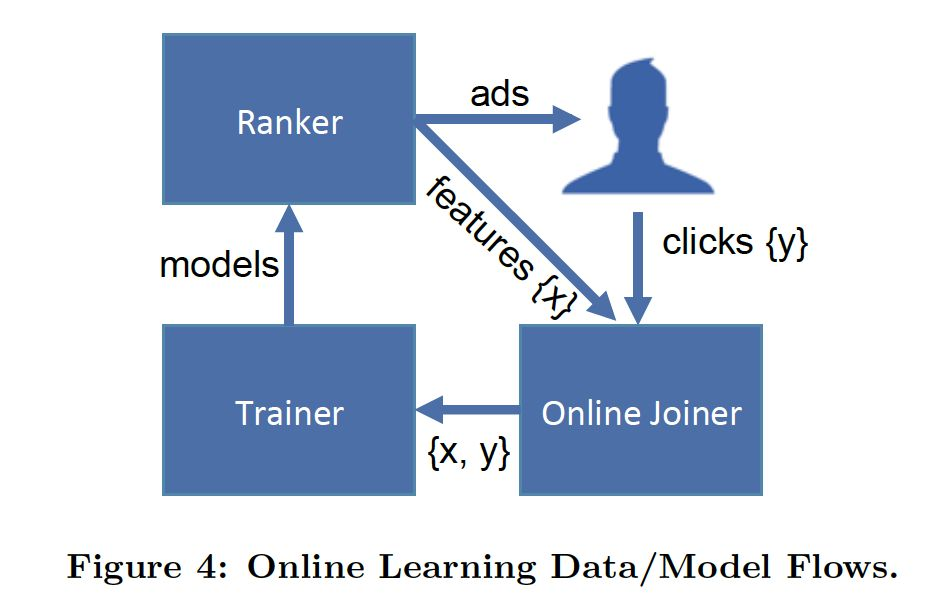
\includegraphics[width=.6\textwidth]{fig/Facebook_Online_Data_Joiner.jpg}
\end{figure}

该模块最重要的作用是准实时的把来自不同数据流的数据整合起来形成sample features,并最终与click数据进行join,形成完整的labeled sample。在整个过程中,我认为最应该注意的有三点:

(1). \textbf{waiting window的设定}:waiting window指的是在impression发生后,我们要等待多久才能够判定一个impression是否有click。如果waiting window过大,数据实时性受影响,如果waiting window过小,会有一部分click来不及join到impression,导致样本CTR与真实值不符。这是一个工程调优的问题,需要有针对性的找到跟实际业务匹配的合适的waiting window。除此之外,无论怎样我们都会漏掉一部分click,这就要求我们阶段性的全量retrain我们的模型,避免online learning误差的积累。

(2). \textbf{分布式的架构与全局统一的action id}:为了实现分布式架构下impression记录和click记录的join,facebook除了为每个action建立全局统一的request id外,还建立了HashQueue缓存impressions。hashQueue缓存的impression,如果在窗口过期时还没有匹配到click就会当作negative sample,这里说的窗口与上面提到的waiting window相匹配。facebook使用scribe实现了这一过程,更多公司使用Kafka完成大数据缓存和流处理。

(3). \textbf{数据流保护机制}:facebook专门提到了online data joiner的保护机制,因为\textcolor{red}{一旦data joiner失效,比如click stream无法join impression stream,那么所有的样本都会成为负样本,由于模型实时进行online learning和serving,模型准确度将立刻受到错误样本数据的影响,进而直接影响广告投放和公司利润,后果是非常严重的}。为此,facebook专门设立了异常检测机制,一旦发现实时样本数据流的分布发生变化,将立即切断online learning的过程,防止预测模型受到影响。

\subsection{降采样和模型校正}
对于巨型互联网公司来说,为了控制数据规模,降低训练开销,降采样几乎是通用的手段,facebook实践了两种降采样的方法,uniform subsampling和 negative down sampling

uniform subsampling是对所有样本进行无差别的随机抽样,为选取最优的采样频率,facebook试验了0.001,0.01, 0.1, 0.5 和1五个采样频率,loss的比较如下:
\begin{figure}[H]
    \centering
    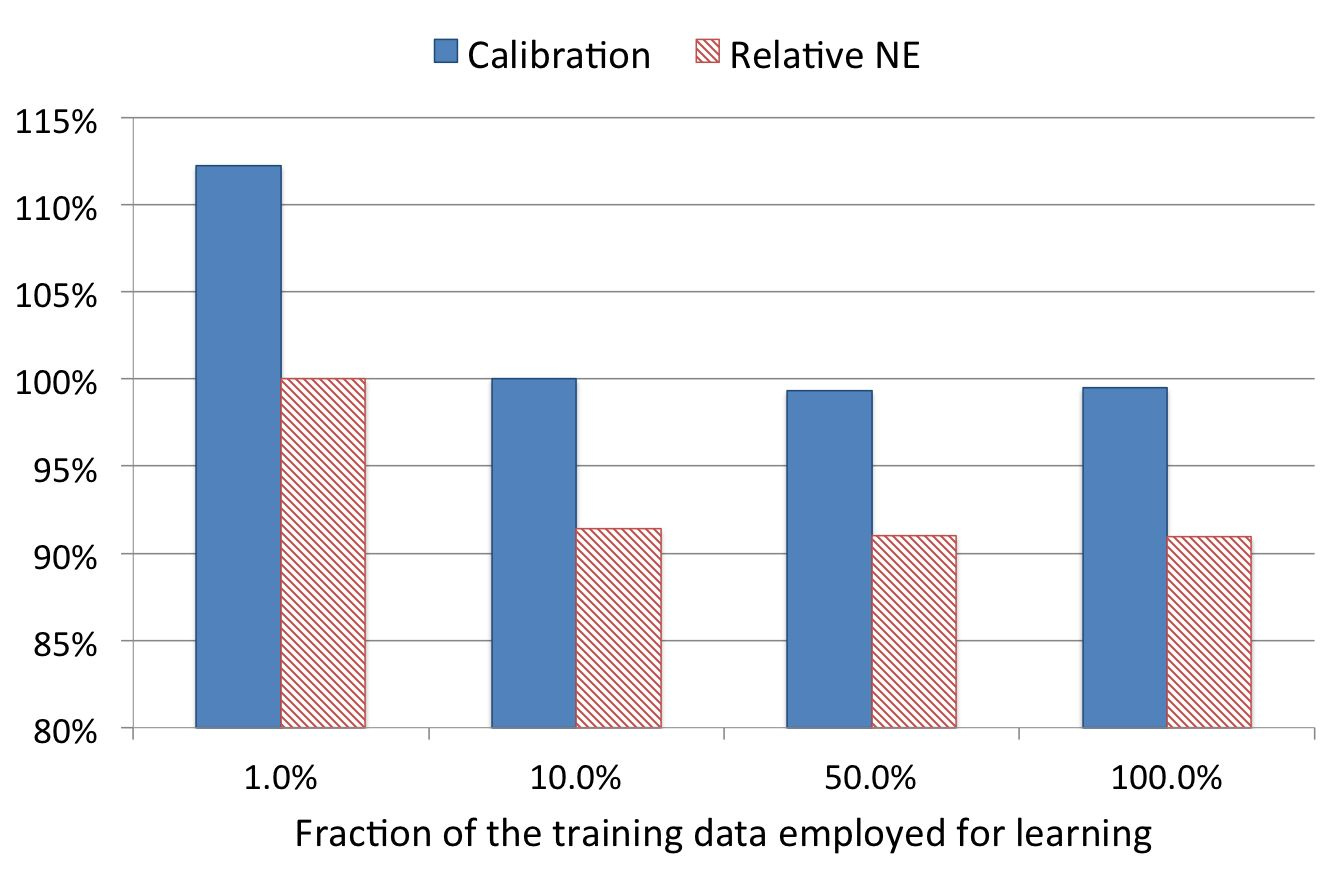
\includegraphics[width=.6\textwidth]{fig/Facebook_DownSample.jpg}
\end{figure}
可以看到当采样率是10%时,相比全量数据训练的模型,仅损失了不到1%的效果。

另一种方法 negative down sampling 保留全量正样本,对负样本进行降采样。除了提高训练效率外,负采样还直接解决了正负样本不均衡的问题,facebook经验性的选择了从0.0001到0.1的一组负采样频率,试验效果如下:
\begin{figure}[H]
    \centering
    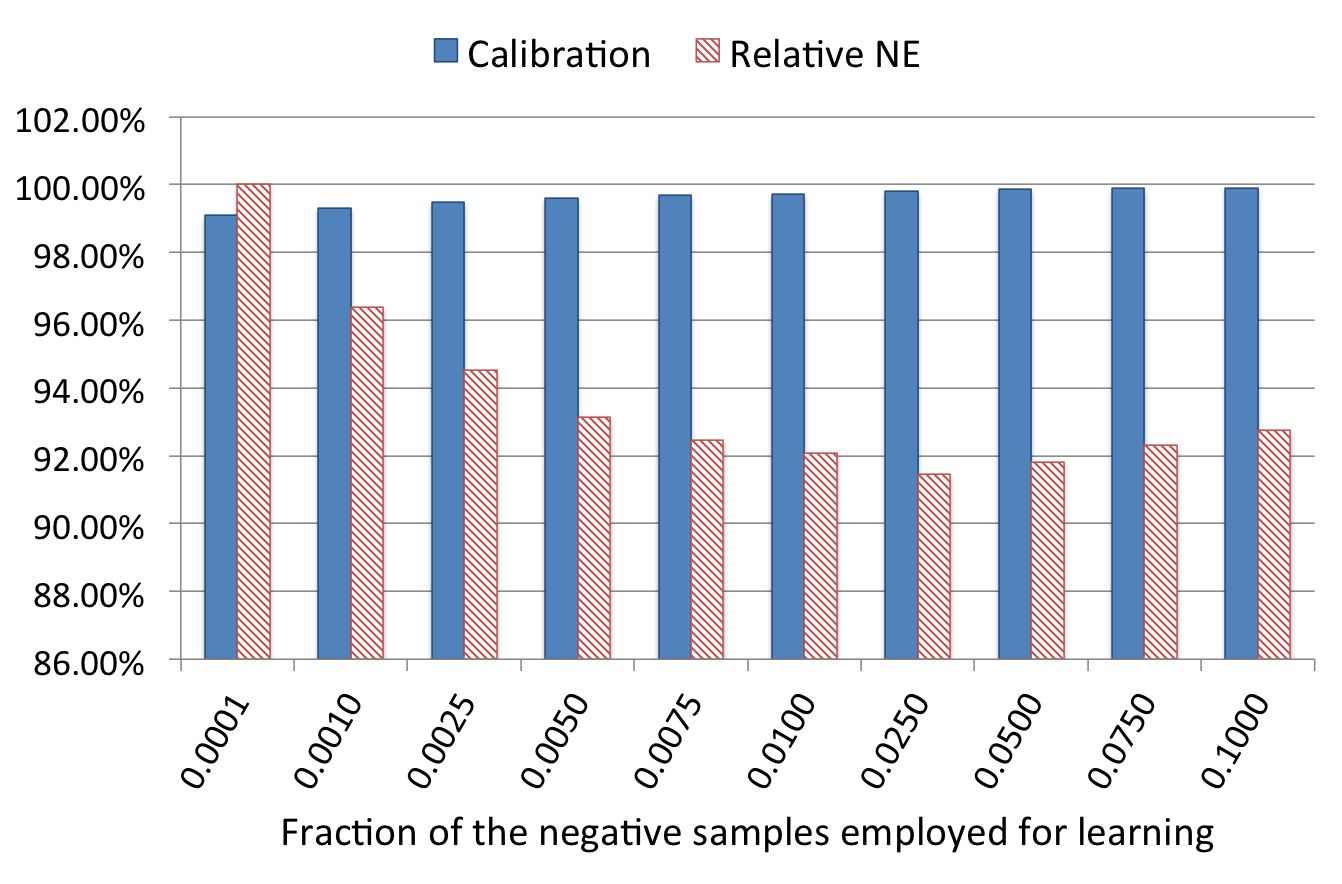
\includegraphics[width=.6\textwidth]{fig/Facebook_Negative_Down_Sampling.jpg}
\end{figure}
大家可以看到,当负采样频率在0.025时,loss不仅优于更低的采样频率训练出来的模型,居然也优于负采样频率在0.1时训练出的模型,虽然原文没有作出进一步的解释,但推测最可能的原因是解决了数据不均衡问题带来的效果提升。

\textbf{负采样带来的问题是CTR预估值的漂移},比如真实CTR是0.1\%,进行0.01的负采样之后,CTR将会攀升到10\%左右。而为了进行准确的竞价以及ROI预估等,CTR预估模型是要提供准确的有物理意义的CTR值的,因此在进行负采样后需要进行CTR的校正,使CTR模型的预估值的期望回到0.1\%。校正的公式如下:
$$
q = \frac{p}{p + (1-p)/w}
$$

其中q是校正后的CTR,p是模型的预估CTR,w是负采样频率。大家可以利用简单的转换关系就可以得出上述公式,有兴趣的同学可以手动推导一下。

\section{Facebook的DLRM模型}
论文:Deep Learning Recommendation Model for Personalization and Recommendation Systems

\subsection{模型架构}
\begin{figure}[H]
    \centering
    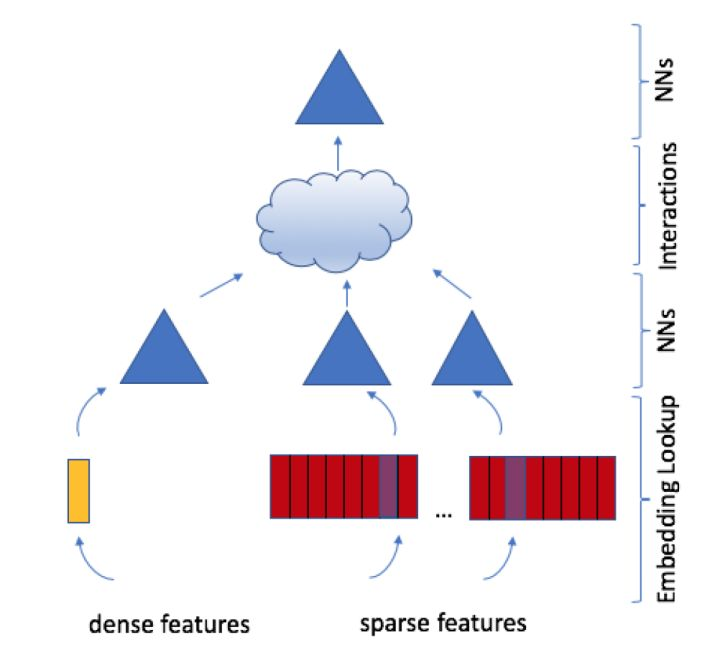
\includegraphics[width=.6\textwidth]{fig/Facebook_DLRM_Structure.jpg}
\end{figure}

从下到上来解释一下Facebook DLRM这个模型的模型结构:
\begin{itemize}
\setlength{\itemsep}{0pt}
\setlength{\parsep}{0pt}
\setlength{\parskip}{0pt}
    \item \textbf{特征工程}:所有特征被分为两类,一类是将类别、id类特征用one hot编码生成的稀疏特征(sparse features),一类是数值型连续特征(dense features)
    \item \textbf{Embedding层}:每个类别类特征转换成one hot vector后,用embedding层转换成维度为 $n$ 的embedding。也就是说,每种稀疏特征转换成一个embedding向量。而年龄、收入等连续型特征将被concat成一个特征向量后,输入图中黄色的MLP(Multi Layer Perceptron)中,被转化成同样维度为 $n$ 的向量。至此,无论是类别类稀疏特征,还是连续型特征组成的特征向量在经过Embedding层后,都被转换成了 $n$ 维的embedding向量。
    \item \textbf{NNs层}:Embedding再往上是由三角形代表的MLP神经网络层,也就是说得到n维的embedding 向量后,每类embedding还有可能进一步通过MLP做转换,原文中这么说的“ optionally passing them through MLPs”,就是说选择性的通过MLP做进一步转换,看来那三个三角形其实是根据调参情况可有可无的。
    \item \textbf{interactions层}:这一层其实这篇文章相对还算创新的一点,它是怎么做的呢?原文这么说的:This is done by taking the dot product between all pairs of embedding vectors and processed dense features. These dot products are concatenated with the original processed dense features and post-processed with another MLP (the top or output MLP)。也就是说会将之前的 embedding 两两做点积,做完之后再跟之前dense features对应的embedding concat起来,喂给后续的MLP。所以这一步其实是希望特征之间做充分的交叉,组合之后,再进入上层MLP做最终的目标拟合。这一点其实follow了FM的特征交叉概念。
    \item 最上层那个三角不用多说,是另一个FC NN,并最终用sigmoid函数给出最终的点击率预估。
\end{itemize}

整个模型看下来,没有特别fancy的结构,也没有加入sequential model,RF等模型的思路,可以说是一个工业界的标准深度学习模型。facebook的博客上还给出了稍微详细一点的模型结构图,大家可以参考。
\begin{figure}[H]
    \centering
    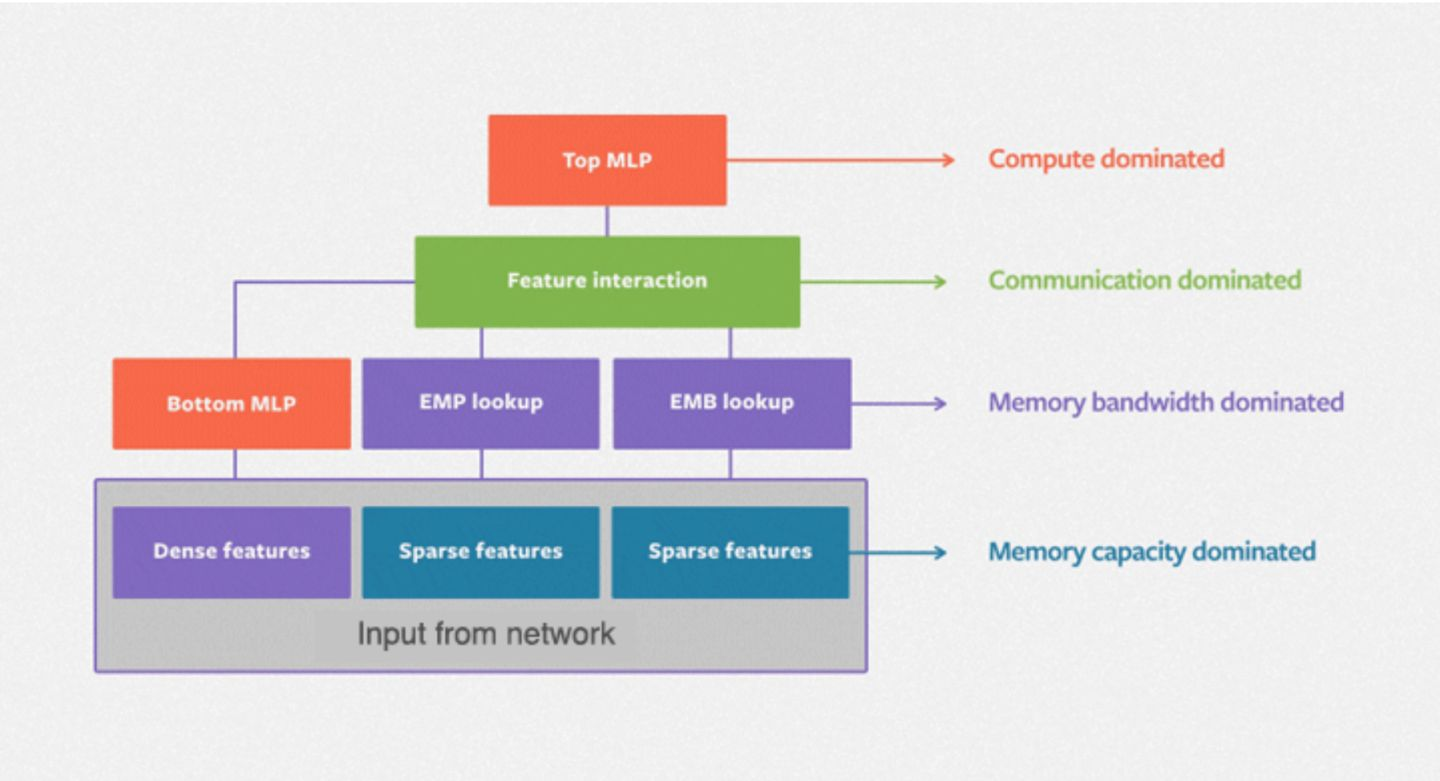
\includegraphics[width=.6\textwidth]{fig/Facebook_DLRM_Structure_Detail.jpg}
\end{figure}

\subsection{Facebook的模型并行训练方法}
作为一篇业界的论文,模型的实际训练方法,训练平台往往是让人受益最多的。而对于Facebook的数据量来说,单节点的模型训练必然无法快速完成任务,那么模型的并行训练就肯定是少不了的解决方法。我们先看原文是如何解释DLRM这个模型的并行训练过程的:

Our parallelized DLRM will use a combination of model parallelism for the embeddings and data parallelism for the MLPs to mitigate the memory bottleneck produced by the embeddings while parallelizing the forward and backward propagations over the MLPs.

简单来说,DLRM融合使用了模型并行和数据并行的方法,对于Embedding部分采用了模型并行,对于MLP部分采用了数据并行。Embedding部分采用模型并行的原因是减轻大量Embedding参数带来的内存瓶颈问题。MLP部分采用数据并行是可以并行进行前向和反向传播。

其实原文中并没有给出非常准确的并行训练方法,这里凭我自己的理解进一步解释一下Embedding做模型并行训练和上层MLP做数据并行训练的原理,对pytorch和caffe2熟悉的专家可以随时纠正我的解释:
\begin{itemize}
\setlength{\itemsep}{0pt}
\setlength{\parsep}{0pt}
\setlength{\parskip}{0pt}
    \item Embedding做模型并行训练指的是在一个device或者说计算节点上,仅有一部分Embedding层参数,每个device进行并行mini batch梯度更新时,仅更新自己节点上的部分Embedding层参数。
    \item MLP层和interactions进行数据并行训练指的是每个device上已经有了全部模型参数,每个device上利用部分数据计算gradient,再利用allreduce的方法汇总所有梯度进行参数更新。
\end{itemize}

\begin{figure}[H]
    \centering
    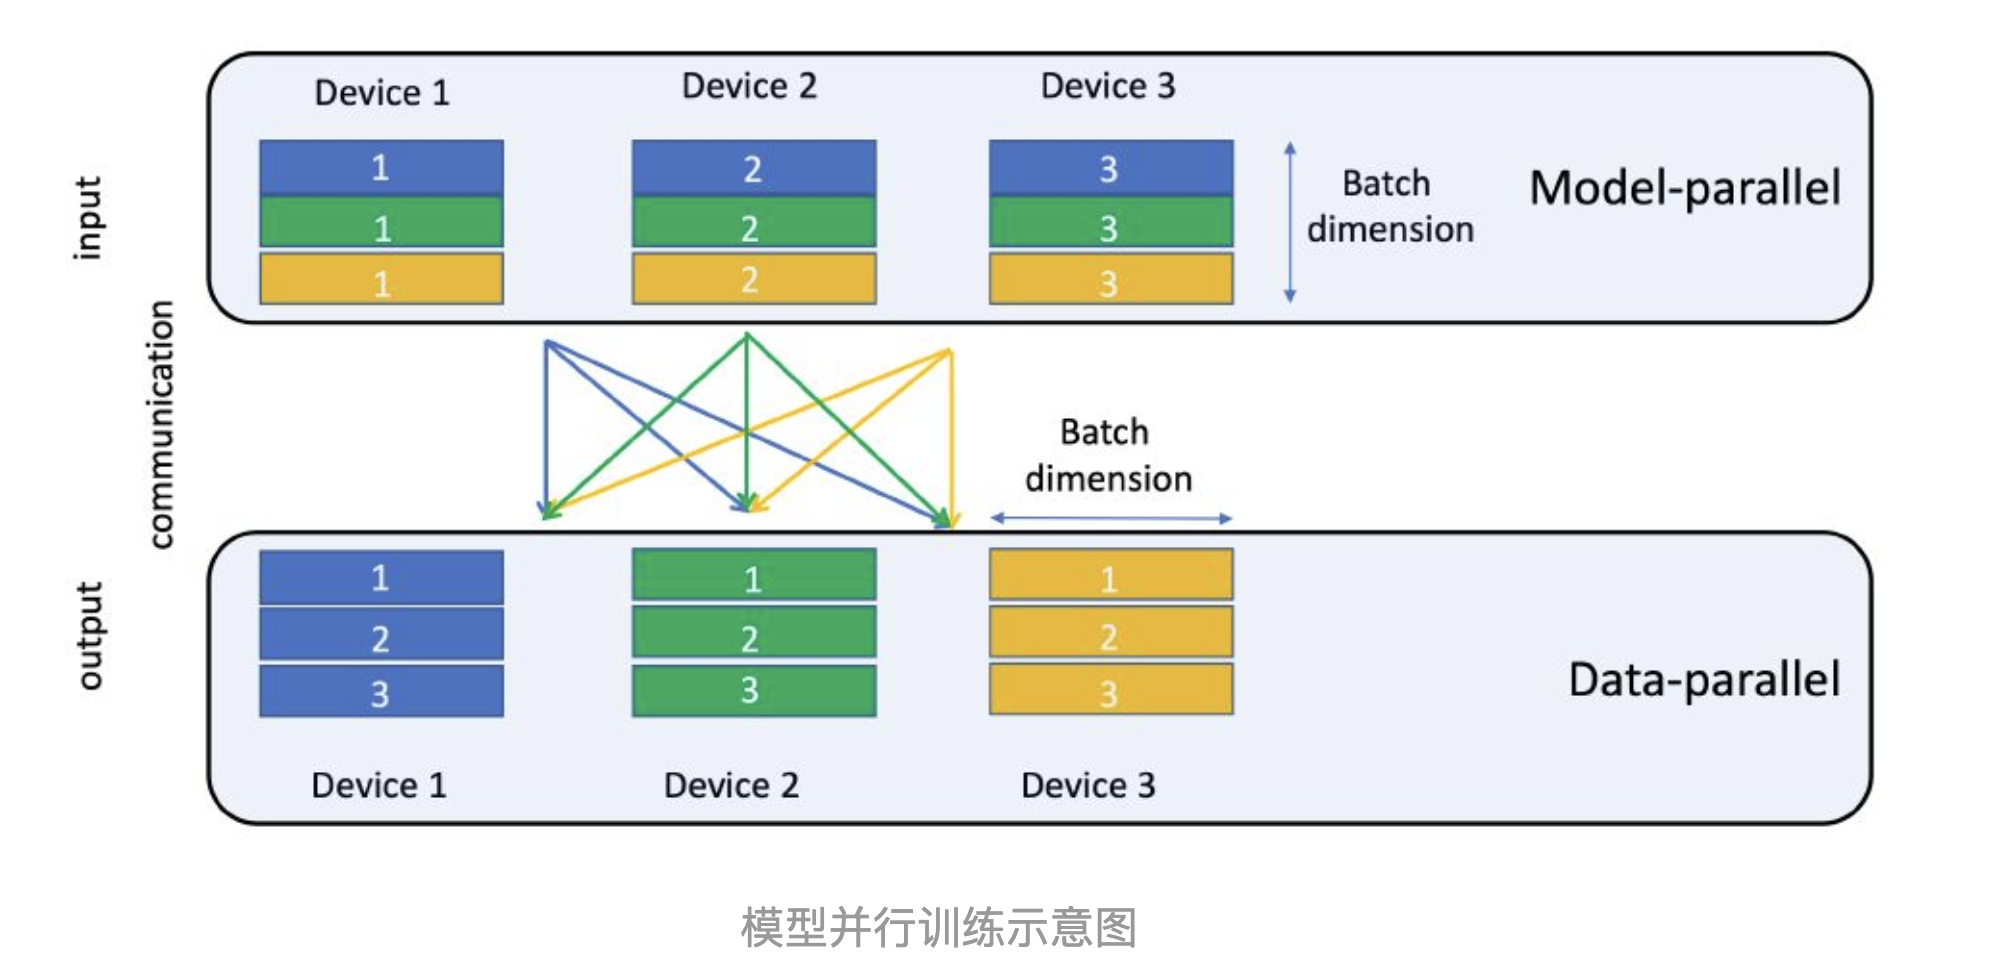
\includegraphics[width=1\textwidth]{fig/Facebook_Parallel_Training.png}
    \caption{模型并行训练示意图}
\end{figure}

\subsection{DLRM模型的效果}
在性能的对比上,DLRM选择了Google 2017年的DCN(Deep cross network)作为baseline。
\begin{figure}[H]
    \centering
    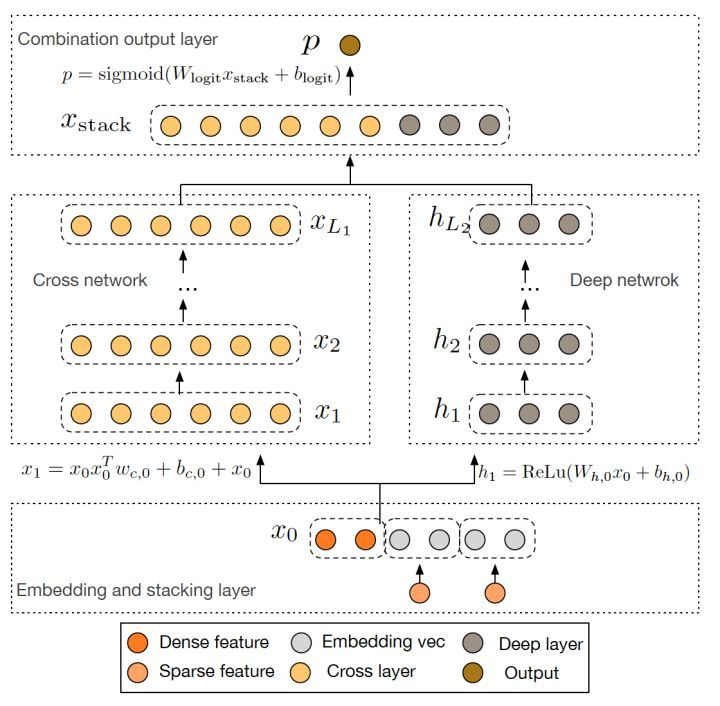
\includegraphics[width=1\textwidth]{fig/Facebook_Google_DCN_Structure.jpg}
    \caption{Google DCN模型结构}
\end{figure}

DCN可以看作是对Wide\&Deep模型的进一步改进,主要的思路使用Cross网络替代了原来的Wide部分。其中设计Cross网络的基本动机是为了增加特征之间的交互力度,使用多层cross layer对输入向量进行特征交叉。单层cross layer的基本操作是将cross layer的输入向量xl与原始的输入向量x0进行交叉,并加入bias向量和原始xl输入向量。

可以看出DLRM和DCN的主要区别在于特征交叉方式的不同,DLRM采用了不同特征域两两点积的交叉方式,DCN采用了每个维度两两交叉的方式。利用Criteo Ad Kaggle data作为测试集,二者的性能对比如下:
\begin{figure}[H]
    \centering
    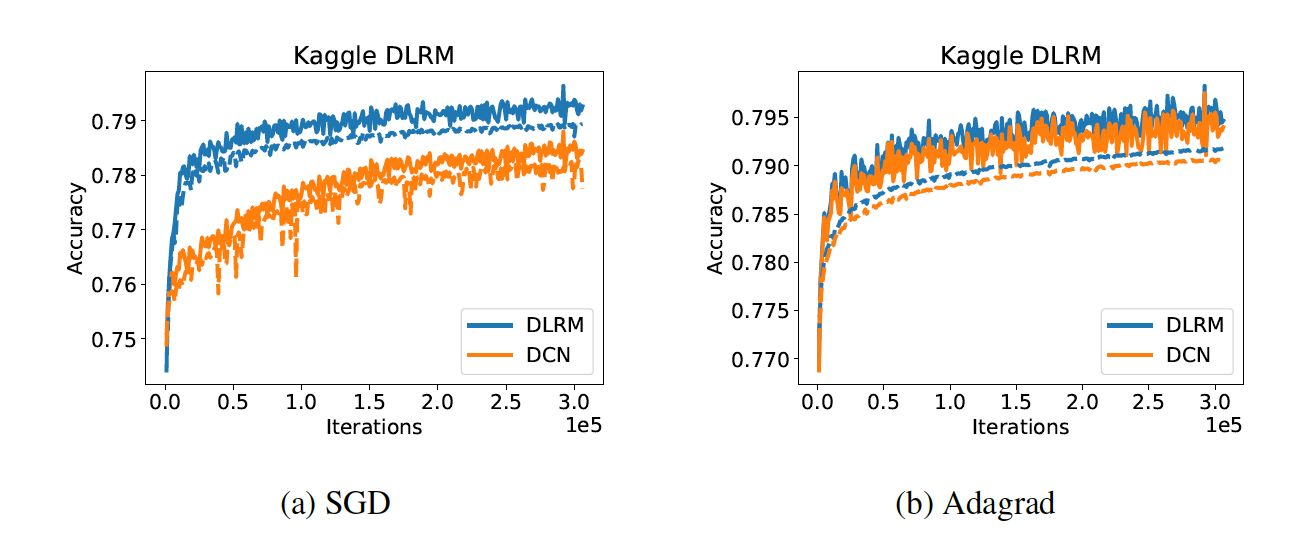
\includegraphics[width=1\textwidth]{fig/Facebook_DLRM_DCN_Compare.jpg}
    \caption{DLRM与DCN性能对比}
\end{figure}

可以看到,DLRM在Accuracy上稍胜一筹。当然模型的performance与数据集的选择,参数的调优都有很大关系。而且DLRM在Adagrad训练方式下的优势已经微乎其微,这里的性能评估大家仅做参考即可。

\section{Youtube的深度学习推荐系统}
论文:Deep Neural Networks for YouTube Recommendations

\subsection{算法基本架构}
Youtube的算法架构如下:
\begin{figure}[H]
    \centering
    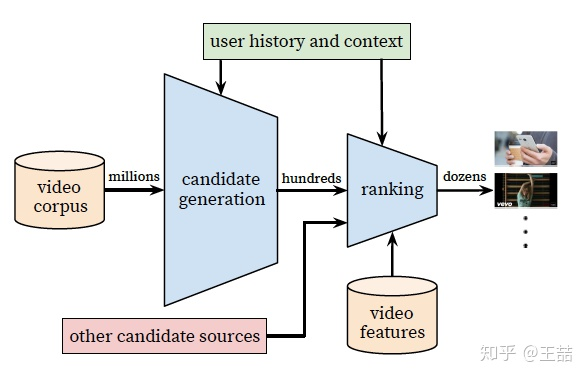
\includegraphics[width=.6\textwidth]{fig/YouTube_Algorithm_Architect.jpg}
\end{figure}

Youtube的用户推荐场景自不必多说,作为全球最大的UGC的视频网站,需要在百万量级的视频规模下进行个性化推荐。由于候选视频集合过大,考虑online系统延迟问题,不宜用复杂网络直接进行推荐,所以Youtube采取了两层深度网络完成整个推荐过程:

(1). 第一层是Candidate Generation Model完成候选视频的快速筛选,这一步候选视频集合由百万降低到了百的量级。

(2). 第二层是用Ranking Model完成几百个候选视频的精排

\subsection{召回层}
首先介绍candidate generation模型的架构:
\begin{figure}[H]
    \centering
    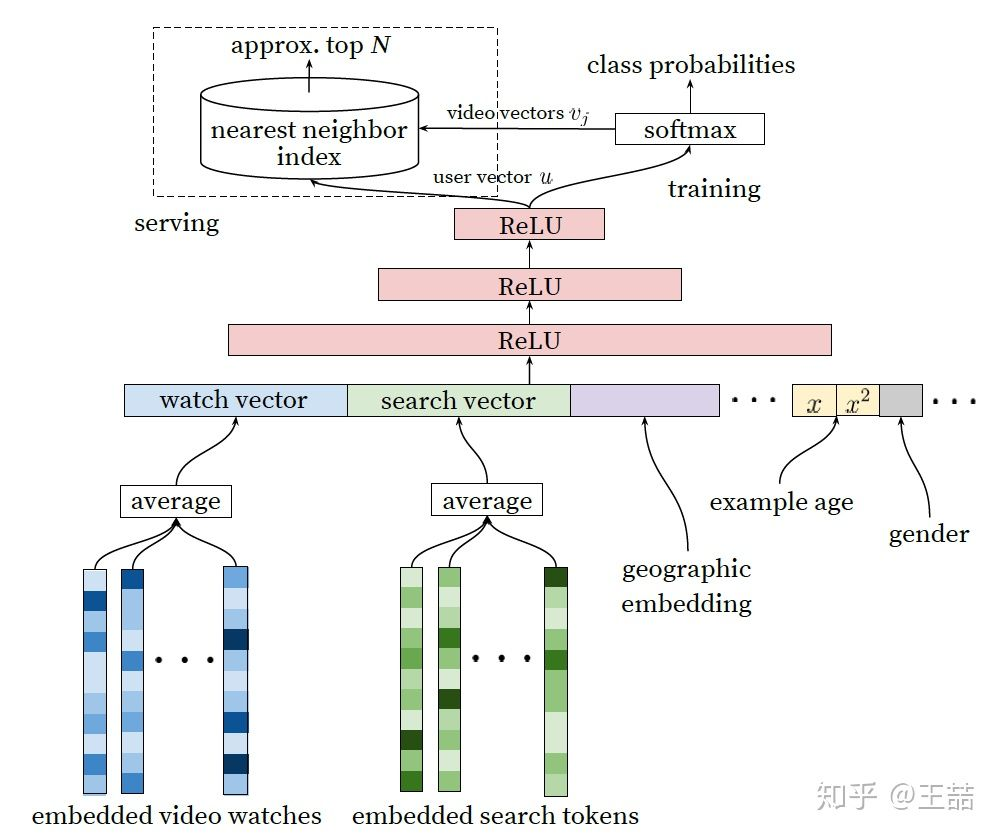
\includegraphics[width=.8\textwidth]{fig/Youtube_Candidate_Generation_Model.jpg}
\end{figure}

我们自底而上看这个网络,最底层的输入是用户观看过的video的embedding向量,以及搜索词的embedding向量。至于这个embedding向量是怎么生成的,作者的原话是这样的

Inspired by continuous bag of words language models, we learn high dimensional embeddings for each video in a fixed vocabulary and feed these embeddings into a feedforward neural network

所以作者是先用word2vec方法对video和search token做了embedding之后再作为输入的,这也是做embedding的“基本操作”,不用过多介绍;当然,除此之外另一种大家应该也比较熟悉,就是通过加一个embedding层跟上面的DNN一起训练,两种方法孰优孰劣,有什么适用场合,大家可以讨论一下。

特征向量里面还包括了用户的地理位置的embedding,年龄,性别等。然后把所有这些特征concatenate起来,喂给上层的ReLU神经网络。

三层神经网络过后,我们看到了softmax函数。这里Youtube的同学们把这个问题看作为用户推荐next watch的问题,所以输出应该是一个在所有candidate video上的概率分布,自然是一个\textbf{多分类}问题。

\subsection{排序层}
既然得到了几百个候选集合,下一步就是利用ranking模型进行精排序,下面是ranking深度学习网络的架构图。
\begin{figure}[H]
    \centering
    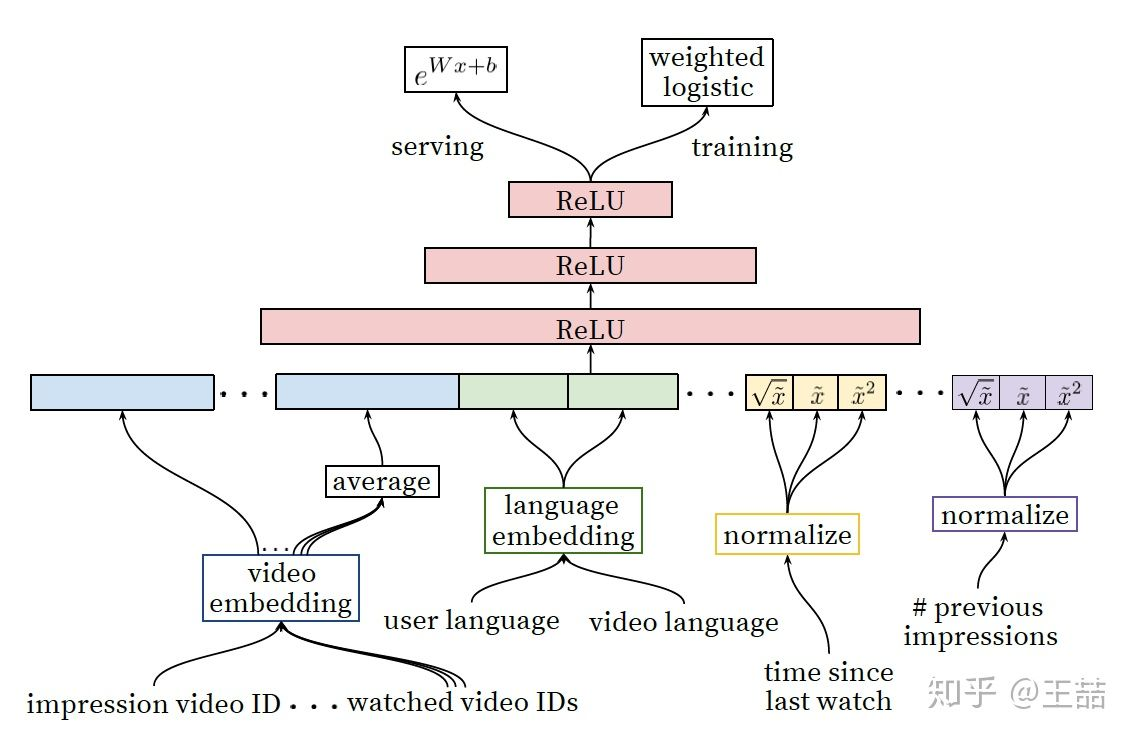
\includegraphics[width=.8\textwidth]{fig/Youtube_Ranking_Model.jpg}
\end{figure}

乍一看上面的ranking model似乎与candidate generation模型没有什么区别,模型架构还是深度学习的“基本操作”,唯一的区别就是特征工程,那么我们就讲讲特征工程。

事实上原文也明确说明了,引入另一套DNN作为ranking model的目的就是引入更多描述视频、用户以及二者之间关系的特征,达到对候选视频集合准确排序的目的。

During ranking, we have access to many more features describing the video and the user's relationship to the video because only a few hundred videos are being scored rather than the millions scored in candidate generation.

具体一点,从左至右的特征依次是
\begin{itemize}
\setlength{\itemsep}{0pt}
\setlength{\parsep}{0pt}
\setlength{\parskip}{0pt}
    \item impression video ID embedding: 当前要计算的video的embedding
    \item watched video IDs average embedding: 用户观看过的最后N个视频embedding的average pooling
    \item language embedding: 用户语言的embedding和当前视频语言的embedding
    \item time since last watch: 自上次观看同channel视频的时间
    \item \#previous impressions: 该视频已经被曝光给该用户的次数
\end{itemize}

上面五个特征中,我想重点谈谈第4个和第5个。因为这两个很好的引入了对用户行为的观察。

第4个特征背后的思想是:We observe that the most important signals are those that describe a user's previous interaction with the item itself and other similar items.

有一些引入attention的意思,这里是用了time since last watch这个特征来反应用户看同类视频的间隔时间。从用户的角度想一想,假如我们刚看过“DOTA经典回顾”这个channel的视频,我们很大概率是会继续看这个channel的视频的,那么该特征就很好的捕捉到了这一用户行为。

第5个特征\#previous impressions则一定程度上引入了exploration的思想,避免同一个视频持续对同一用户进行无效曝光。尽量增加用户没看过的新视频的曝光可能性。

\subsection{工程实践}
\subsubsection{softmax的训练}
文中把推荐问题转换成多分类问题,在预测next watch的场景下,每一个备选video都会是一个分类,因此总共的分类有数百万之巨,这在使用softmax训练时无疑是低效的,这个问题YouTube是如何解决的?

这个问题原文的回答是这样的:We rely on a technique to sample negative classes from the background distribution ("candidate sampling") and then correct for this sampling via importance weighting.

简单说就是进行了负采样(negative sampling)并用importance weighting的方法对采样进行calibration。文中同样介绍了一种替代方法,hierarchical softmax,但并没有取得更好的效果。当然关于采样的具体技术细节以及优劣可能再开一篇文章都讲不完,感兴趣的同学可以参考tensorflow中的介绍(\url{https://www.tensorflow.org/extras/candidate_sampling.pdf})以及NLP领域的经典论文 \url{http://www.aclweb.org/anthology/P15-1001}

\subsubsection{最近邻搜索}
在candidate generation model的serving过程中,YouTube为什么不直接采用训练时的model进行预测,而是采用了一种最近邻搜索的方法?

这个问题的答案是一个经典的工程和学术做trade-off的结果,在model serving过程中对几百万个候选集逐一跑一遍模型的时间开销显然太大了,因此在通过candidate generation model得到user 和 video的embedding之后,通过最近邻搜索的方法的效率高很多。我们甚至不用把任何model inference的过程搬上服务器,只需要把user embedding和video embedding存到redis或者内存中就好了。

\subsubsection{新视频的偏好特征}
Youtube的用户对新视频有偏好,那么在模型构建的过程中如何引入这个feature?

为了拟合用户对fresh content的bias,模型引入了“Example Age”这个feature,文中其实并没有精确的定义什么是example age。按照文章的说法猜测的话,会直接把sample log距离当前的时间作为example age。比如24小时前的日志,这个example age就是24。在做模型serving的时候,不管使用那个video,会直接把这个feature设成0。大家可以仔细想一下这个做法的细节和动机,非常有意思。

当然我最初的理解是训练中会把Days since Upload作为这个example age,比如虽然是24小时前的log,但是这个video已经上传了90小时了,那这个feature value就是90。那么在做inference的时候,这个feature就不会是0,而是当前时间每个video的上传时间了。

我不能100\%确定文章中描述的是那种做法,大概率是第一种。还请大家踊跃讨论。

文章也验证了,example age这个feature能够很好的把视频的freshness的程度对popularity的影响引入模型中。

\subsubsection{采样训练样本}
在对训练集的预处理过程中,YouTube没有采用原始的用户日志,而是对每个用户提取等数量的训练样本,这是为什么?

原文的解答是这样的:Another key insight that improved live metrics was to generate a fixed number of training examples per user, effectively weighting our users equally in the loss function. This prevented a small cohort of highly active users from dominating the loss. 理由很简单,这是为了减少高度活跃用户对于loss的过度影响。

\subsubsection{历史的时序特征}
YouTube为什么不采取类似RNN的Sequence model,而是完全摒弃了用户观看历史的时序特征,把用户最近的浏览历史等同看待,这不会损失有效信息吗?

这个原因应该是YouTube工程师的“经验之谈”,如果过多考虑时序的影响,用户的推荐结果将过多受最近观看或搜索的一个视频的影响。YouTube给出一个例子,如果用户刚搜索过“tayer swift”,你就把用户主页的推荐结果大部分变成tayer swift有关的视频,这其实是非常差的体验。为了综合考虑之前多次搜索和观看的信息,YouTube丢掉了时序信息,讲用户近期的历史纪录等同看待。

但RNN到底适不适合next watch这一场景,其实还有待商榷,目前youtube已经上线了以RNN为基础的推荐模型, 参考论文如下: \url{https://static.googleusercontent.com/media/research.google.com/en//pubs/archive/46488.pdf}

\subsubsection{生成测试集}
在处理测试集的时候,YouTube为什么不采用经典的随机留一法(random holdout),而是一定要把用户最近的一次观看行为作为测试集?

这个问题比较好回答,只留最后一次观看行为做测试集主要是为了避免引入future information,产生与事实不符的数据穿越。

\subsubsection{优化目标}
在确定优化目标的时候,YouTube为什么不采用经典的CTR,或者播放率(Play Rate),而是采用了每次曝光预期播放时间(expected watch time per impression)作为优化目标?

这个问题从模型角度出发,是因为 watch time更能反应用户的真实兴趣,从商业模型角度出发,因为watch time越长,YouTube获得的广告收益越多。而且增加用户的watch time也更符合一个视频网站的长期利益和用户粘性。

这个问题看似很小,实则非常重要,objective的设定应该是一个算法模型的根本性问题,而且是算法模型部门跟其他部门接口性的工作,从这个角度说,YouTube的推荐模型符合其根本的商业模型,非常好的经验。

\subsubsection{video embedding}
在进行video embedding的时候,为什么要直接把大量长尾的video直接用0向量代替?

这又是一次工程和算法的trade-off,把大量长尾的video截断掉,主要还是为了节省online serving中宝贵的内存资源。当然从模型角度讲,低频video的embedding的准确性不佳是另一个“截断掉也不那么可惜”的理由。

当然,之前很多同学在评论中也提到简单用0向量代替并不是一个非常好的选择,那么有什么其他方法,大家可以思考一下。

\subsubsection{特征的特殊处理}
针对某些特征,比如\#previous impressions,为什么要进行开方和平方处理后,当作三个特征输入模型?

这是很简单有效的工程经验,引入了特征的非线性。从YouTube这篇文章的效果反馈来看,提升了其模型的离线准确度。

\subsubsection{输出层}
为什么ranking model不采用经典的logistic regression当作输出层,而是采用了weighted logistic regression?

因为在第7问中,我们已经知道模型采用了expected watch time per impression作为优化目标,所以如果简单使用LR就无法引入正样本的watch time信息。因此采用weighted LR,将watch time作为正样本的weight,在线上serving中使用e(Wx+b)做预测可以直接得到expected watch time的近似,完美。

\subsection{详细解读输出层采用 weighted logistic regression}

对于传统的深度学习架构,输出层往往采用LR或者Softmax,在线上预测过程中,也是原封不动的照搬LR或者softmax的经典形式来计算点击率(广义地说,应该是正样本概率)。

而YouTube这一模型的神奇之处在于,输出层没有使用LR,而是采用了Weighted LR,模型serving没有采用sigmoid函数的形式,而是使用了
$e^{Wx+b}$这一指数形式。按照原文说法,这样做预测的就是用户观看时长??

搞清楚这件事情并不是一件容易的事情,我们要从逻辑回归的本质意义上开始。

几乎所有算法工程师的第一堂课就是逻辑回归,也肯定知道逻辑回归的数学形式就是一个线性回归套sigmoid函数:
$$
h_\theta(x) = \frac{1}{1+e^{-\theta^Tx}}
$$

但为什么选择sigmoid函数?难道仅仅是sigmoid函数能把值域映射到0-1之间,符合概率的物理意义这么简单吗?

为解释这个问题,首先我们需要定义一个新的变量——Odds,中文可以叫发生比或者机会比。
$$
Odds = \frac{p}{1-p}
$$

假设一件事情发生的概率是p,那么\textbf{Odds就是一件事情发生和不发生的比值}。

如果对Odds取自然对数,再让ln(Odds)等于一个线性回归函数,那么就得到了下面的等式。
$$
logit(p) = \ln(\frac{p}{1-p}) = \theta_0 + \theta_1x_1 + \theta_2x_2
$$

其中$\ln(p/(1-p))$就是大名鼎鼎的logit函数,logistics regression又名logit regression,上面的式子就是逻辑回归的由来。我们再做进一步运算,就可以转变成我们熟悉的逻辑回归的形式:
$$
 \ln(\frac{p}{1-p}) = \theta^Tx \Rightarrow \frac{p}{1-p} = e^{\theta^Tx} \Rightarrow p = \frac{1}{1+e^{-\theta^Tx}} \Rightarrow p = sigmoid(\theta^Tx)
$$

到这里大家应该已经完全明白了LR的推导过程了。

那么再对$\ln(Odds) = \theta^Tx$这个等式做一个小小的转换,两边取自然底数:
$$
\ln(Odds) = \theta^Tx \Rightarrow Odds = e^{\theta^Tx} = YouTubeServingFunction
$$

大家看到了吗,\textbf{Youtube的Serving函数$e^{Wx+b}$计算的不是别的,正是Odds}!

但我们还没有到达终点,因为Youtube要预测的明明是用户观看时长,怎么就成了Odds了?

这就要提到YouTube采用的独特的训练方式Weighted LR,这里的Weight,对于正样本$i$来说就是观看时长$T_i$,对于负样本来说,则指定了单位权重1。

Weighted LR的特点是,正样本权重$w$的加入会让正样本发生的几率变成原来的$w$倍,也就是说样本i的Odds变成了下面的式子:
$$
Odds(i) = \frac{w_ip}{1-w_ip}
$$

由于在视频推荐场景中,用户打开一个视频的概率p往往是一个很小的值,因此上式可以继续简化:
$$
Odds(i) = \frac{w_ip}{1-w_ip} \approx w_ip = T_ip = E(T_i)
$$

而且由于YouTube采用了用户观看时长$T_i$作为权重,因此式子进一步等于$T_i*p$,这里真相就大白了,由于$p$就是用户打开视频的概率,$T_i$是观看时长,因此$T_i*p$就是用户观看某视频的期望时长!

因此,YouTube采用$e^{Wx+b}$ 这一指数形式预测的就是曝光这个视频时,用户观看这个视频的时长的期望!利用该指标排序后再进行推荐,是完全符合YouTube的推荐场景和以观看时长为优化目标的设定的。


\textbf{再简要总结一下YouTube Ranking Model的Serving过程要点}

(1) $e^{Wx+b}$  这一指数形式计算的是Weighted LR的Odds;

(2) Weighted LR使用用户观看时长作为权重,使得对应的Odds表示的就是用户观看时长的期望;

(3) Model Serving过程中$e^{Wx+b}$计算的正是观看时长的期望。

\section{阿里深度兴趣网络(DIN)}
\subsection{用户场景}
用户场景很简单,就是在一个电商网站或APP中给用户推荐广告,当然对于阿里妈妈来说,广告也是商品,所以这篇文章的广告场景其实也是一个经典的推荐场景。

好,既然要推荐,我们当然需要利用用户的历史数据了,对于一个电商来说,历史数据当然就是点击,添加购物车,下单这些行为了。论文中给了一位用户的行为序列。
\begin{figure}[H]
    \centering
    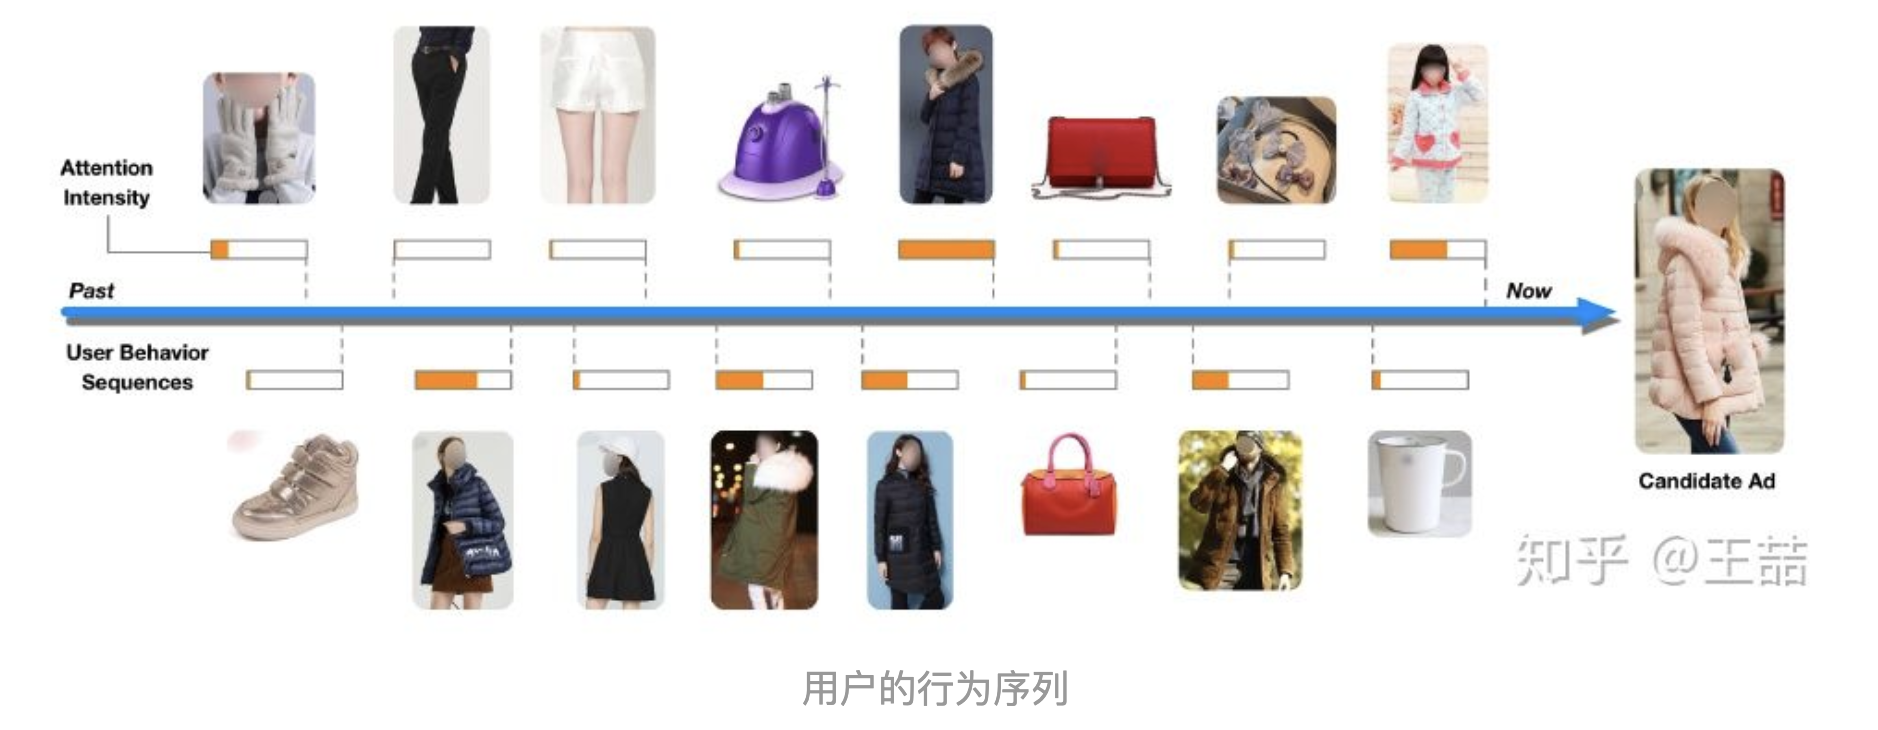
\includegraphics[width=1\textwidth]{fig/Ali_User_Behavior_Sequence.png}
    \caption{用户的行为序列}
\end{figure}

显然是一个女生的行为历史啦,从最左边的手套,鞋子到右边的杯子,睡衣。要被推荐的候选商品是一件女式大衣。我们应该如何计算这件大衣的CTR呢?

\begin{framed}
如果按照之前的做法,我们会一碗水端平的考虑所有行为记录的影响,对应到模型中就是我们会用一个average pooling层把用户交互过的所有商品的embedding vector平均一下形成这个用户的user vector,机灵一点的工程师最多加一个time decay,让最近的行为产生的影响大一些,那就是在做average pooling的时候按时间调整一下权重。

但是我们仔细想一想我们自己的购买过程,其实每个用户的兴趣都是多样的,女生喜欢买衣服包包,也喜欢化妆品,甚至还为自己男朋友挑选过球衣球鞋,那么你在买大衣的时候,真的要把给男朋友买球鞋的偏好考虑进来么?具体到本文的例子中,在预测大衣的CTR这件事情上,用户浏览过杯子,跟用户浏览过另一件大衣这两个行为的重要程度是一样的吗?

这事不用问算法工程师,你就回家问问你老妈估计答案都是一定的,肯定是浏览过另一件大衣这件事的参考价值高啊。好了,就是这件你老妈都知道的事情,让阿里妈妈的算法工程师们加上了attention机制。
\end{framed}

\subsection{注意力机制}
注意力机制顾名思义,就是模型在预测的时候,对用户不同行为的注意力是不一样的,“相关”的行为历史看重一些,“不相关”的历史甚至可以忽略。那么这样的思想反应到模型中也是直观的。
$$
V_u  = f(V_a) = \sum_{i=1}^Nw_i * V_i = \sum_{i=1}^Ng(V_i, V_a) * V_i
$$

其中,$V_u$是用户的 embedding 向量,$V_a$是候选广告商品的 embedding 向量,$V_i$ 是用户$u$的第$i$次行为的 embedding 向量,因为这里用户的行为就是浏览商品或店铺,所以行为的embedding的向量就是那次浏览的商品或店铺的embedding向量。

因为加入了注意力机制,$V_u$ 从过去 $V_i$ 的\textbf{加和}变成了$V_u$ 的\textbf{加权和}, $V_i$ 的权重 $w_i$ 就由 $V_i$ 与 $V_a$ 的关系决定,也就是上式中的 $g(V_i, V_a)$。

那么 $g(V_i, V_a)$ 这个函数到底采用什么比较好呢?看完下面的架构图自然就清楚了。
\begin{figure}[H]
    \centering
    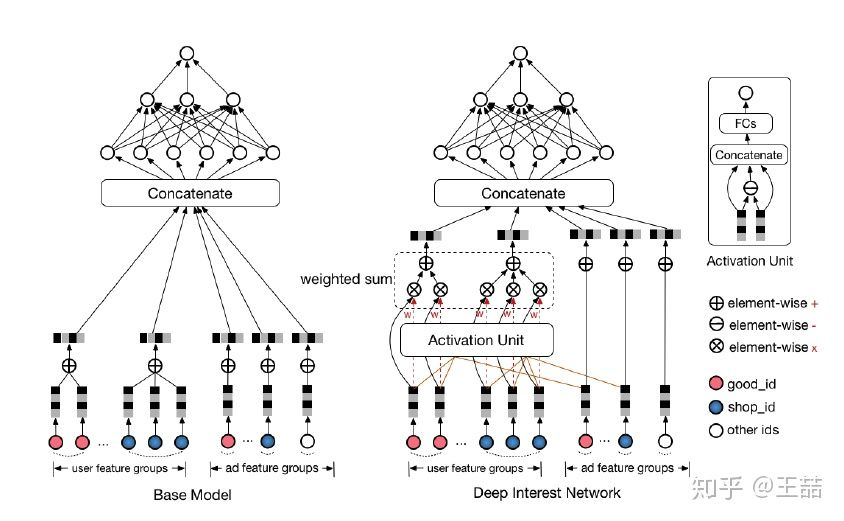
\includegraphics[width=1\textwidth]{fig/Ali_DIN_Structure.jpg}
    \caption{用户的行为序列}
\end{figure}

相比原来这个标准的深度推荐网络(Base model),DIN在生成用户embedding vector的时候加入了一个activation unit层,这一层产生了每个用户行为$V_i$ 的权重,下面我们仔细看一下这个权重是怎么生成的,也就是 $g(V_i, V_a)$ 是如何定义的。

传统的Attention机制中,给定两个item embedding,比如 $u$ 和 $v$,通常是直接做点积 $uv$ 或者 $uWv$,其中 $W$ 是一个 $|u|\times |v|$ 的权重矩阵,但这篇paper中阿里显然做了更进一步的改进,着重看上图右上角的activation unit,\textbf{首先是把 $u$ 和 $v$ 以及 $u v$ 的element wise差值向量合并起来作为输入,然后喂给全连接层,最后得出权重},这样的方法显然损失的信息更少。但如果你自己想方便的引入attention机制的话,不妨先从点积的方法做起尝试一下,因为这样连训练都不用训练。

再稍微留意一下这个架构图中的红线,你会发现每个ad会有 good\_id, shop\_id 两层属性,shop\_id只跟用户历史中的shop\_id序列发生作用,good\_id只跟用户的good\_id序列发生作用,这样做的原因也是显而易见的。

\subsection{论文作者的评论}
其实最初的时候我们不是按照借鉴attention的套路来的,当时想法就是希望做个反向激活的网络结构,能自适应地挑跟candidate相关的用户行为来做用户兴趣的表征,后来写论文的时候仔细survey发现这个是attention的解法。再透露个细节,其实在DL模型之前,我们就研制了一种可以认为是hard模式的attention结构:那是特征组合的解法,我们用ad的shop属性去hit用户历史行为过的shop list,如果命中了那么就说明历史用户有过直接行为,用行为id和频次来表示这个组合特征;如果没有命中特征就是空的,那显然attention结构就是一种自然的soft扩展,不过适用范围更强了

%\printbibliography
\bibliography{../ref}
\bibliographystyle{IEEEtran}
\end{document}